% Chapter 1

\chapter{Deep Polarization-Based Semantic Segmentation} % Main chapter title

\label{Chapter4} % For referencing the chapter elsewhere, use \ref{Chapter1} 

%----------------------------------------------------------------------------------------

% Define some commands to keep the formatting separated from the content 


%----------------------------------------------------------------------------------------

This chapter is dedicated to segmented map estimation from a polarimetric image. As described in Chapter \ref{Chapter2}, segmentation represent a rising field in computer vision. In essence, it is a pixel-level classification of images. Moreover, it is possible to add the semantic dimension to the problem to formulate the interconnections of the classes and to add a part of understanding.

In the framework of the presented work, we propose to use polarization as an input modality. While the vast majority of algorithms rely on so-called standard modalities, such as colorimetry, we want to show a change of space can modify, even simplify, the problem of semantic segmentation of complex urban scenes.
As a consequence of this change of modality, we propose reviewing the whole pipeline from the database to the estimation via CNN through the creation of an adequate augmentation procedure.

This chapter is constituted as follows. We briefly introduce our scenario and motivations in Section \ref{intro_4}. In Section \ref{mod_4}, we discuss the modality constraints as well as the choices made to make the polarization usable. Then, in Section \ref{aug_4}, we focus on the augmentation process. 
Finally, Section \ref{net_4} and Section \ref{exp_4} will respectively discuss the networks used and the experiments.
Section \ref{sum_4} summarizes our work.

\section{Introduction}\label{intro_4}

Recently, pixel-wise semantic segmentation (PwSS) has achieved great success especially thanks to the increased computing capacity of modern machines. Yet, a less expensive solution is very little investigated, the moderate use of data and computing power. The formulation of the problem is then marginally different. Instead of loading the networks with a vast amount of data and/or increasing their size, the problem is estimated upstream to discriminate the network.
It is nevertheless notable some contributions are tackling the problem, such as few-shot learning \cite{dong2018few, siam2019amp}. However, a very small minority transpose the data space to apply a constraint ahead of the network rather than impacting the processing core.

We aim to propose a complete PwSS pipeline to describe complex urban scenes based on polarimetric imagery.Here, "complex" defines the possibility of adverse weather conditions and scenes subject to reflection. We start with an observation: urban scenes are prone to specular relfection. Indeed, whether it is the metallic paint of cars, road signs, the presence of windows or even the road in rainy conditions, these surfaces reflect the light.Rather than defining these reactions in a space that saturates in these cases, we propose to implement a modality in which these phenomena are defined.
We then propose using polarization instead of colorimetry which would export its constraints relative to these occurrences. We therefore rely on polarization to simplify the segmentation problem in urban environments.
Thus, we need deconstructing all the achievements in the PwSS domains to reconstruct a polarization-adapted pipeline: the dataset, the image representation, the augmentation and the estimation of the results.

In practice, the methods require massive datasets like KITTI \cite{Geiger2012CVPR} or Cityscape \cite{Cordts2016Cityscapes} that deliver both corresponding input image with a reference segmented map.
These mass requirements are onerous to achieve when implementing a non-conventional modality, which motivates a more measured use of the data.
A straightforward approach would be to acquire a large amount of data and then annotate it to enrich the generalization capacity of the network. Since our approach is alternative, we propose to acquire a limited number of images and use the augmentation to enrich the set.
Although augmentation has been popularized for its advantages in terms of problem generalization and overfitting prevention, it is only viable for interpolable images. In short, as soon as an image is directly related to the physics of the scene, this process is not applicable since it will alter the validity of the observation. On the other hand, since the colorimetry is interpolable and does not report any alteration as a result of it, then the augmentation is valid for this type of image.
In line with the initial objective of the augmentation, we define a group of transforms applicable to polarimetric imaging and in particular, we focus on the physical adequacy of these.
Since it is necessary to benchmark the proposed solution, we tackle the possibility of evaluating our method and especially in competition with the conventional approaches. Aiming this objective, we have aggregated our dataset taking into account that each polarimetric image and segmentation pair correspond to an RGB image and segmentation pair. 
 
\section{Modality-related constraints}\label{mod_4}

As stated previously and more precisely in the Section \ref{Polar_explain}, with polarization follows a set of constraints of its own.
In this section the numerous constraining items of the modality will be discussed. First, the fomulation of the problem with respect to the data will be stated. Then, in part \ref{rep_pol}, the representation aspect of the imagery will be addressed. This chapter will be concluded by the methods operated to aggregate and validate this dataset.

\begin{figure}[ht]
	\centering
	
	\begin{subfigure}[b]{.8\linewidth}   
		\centering 
		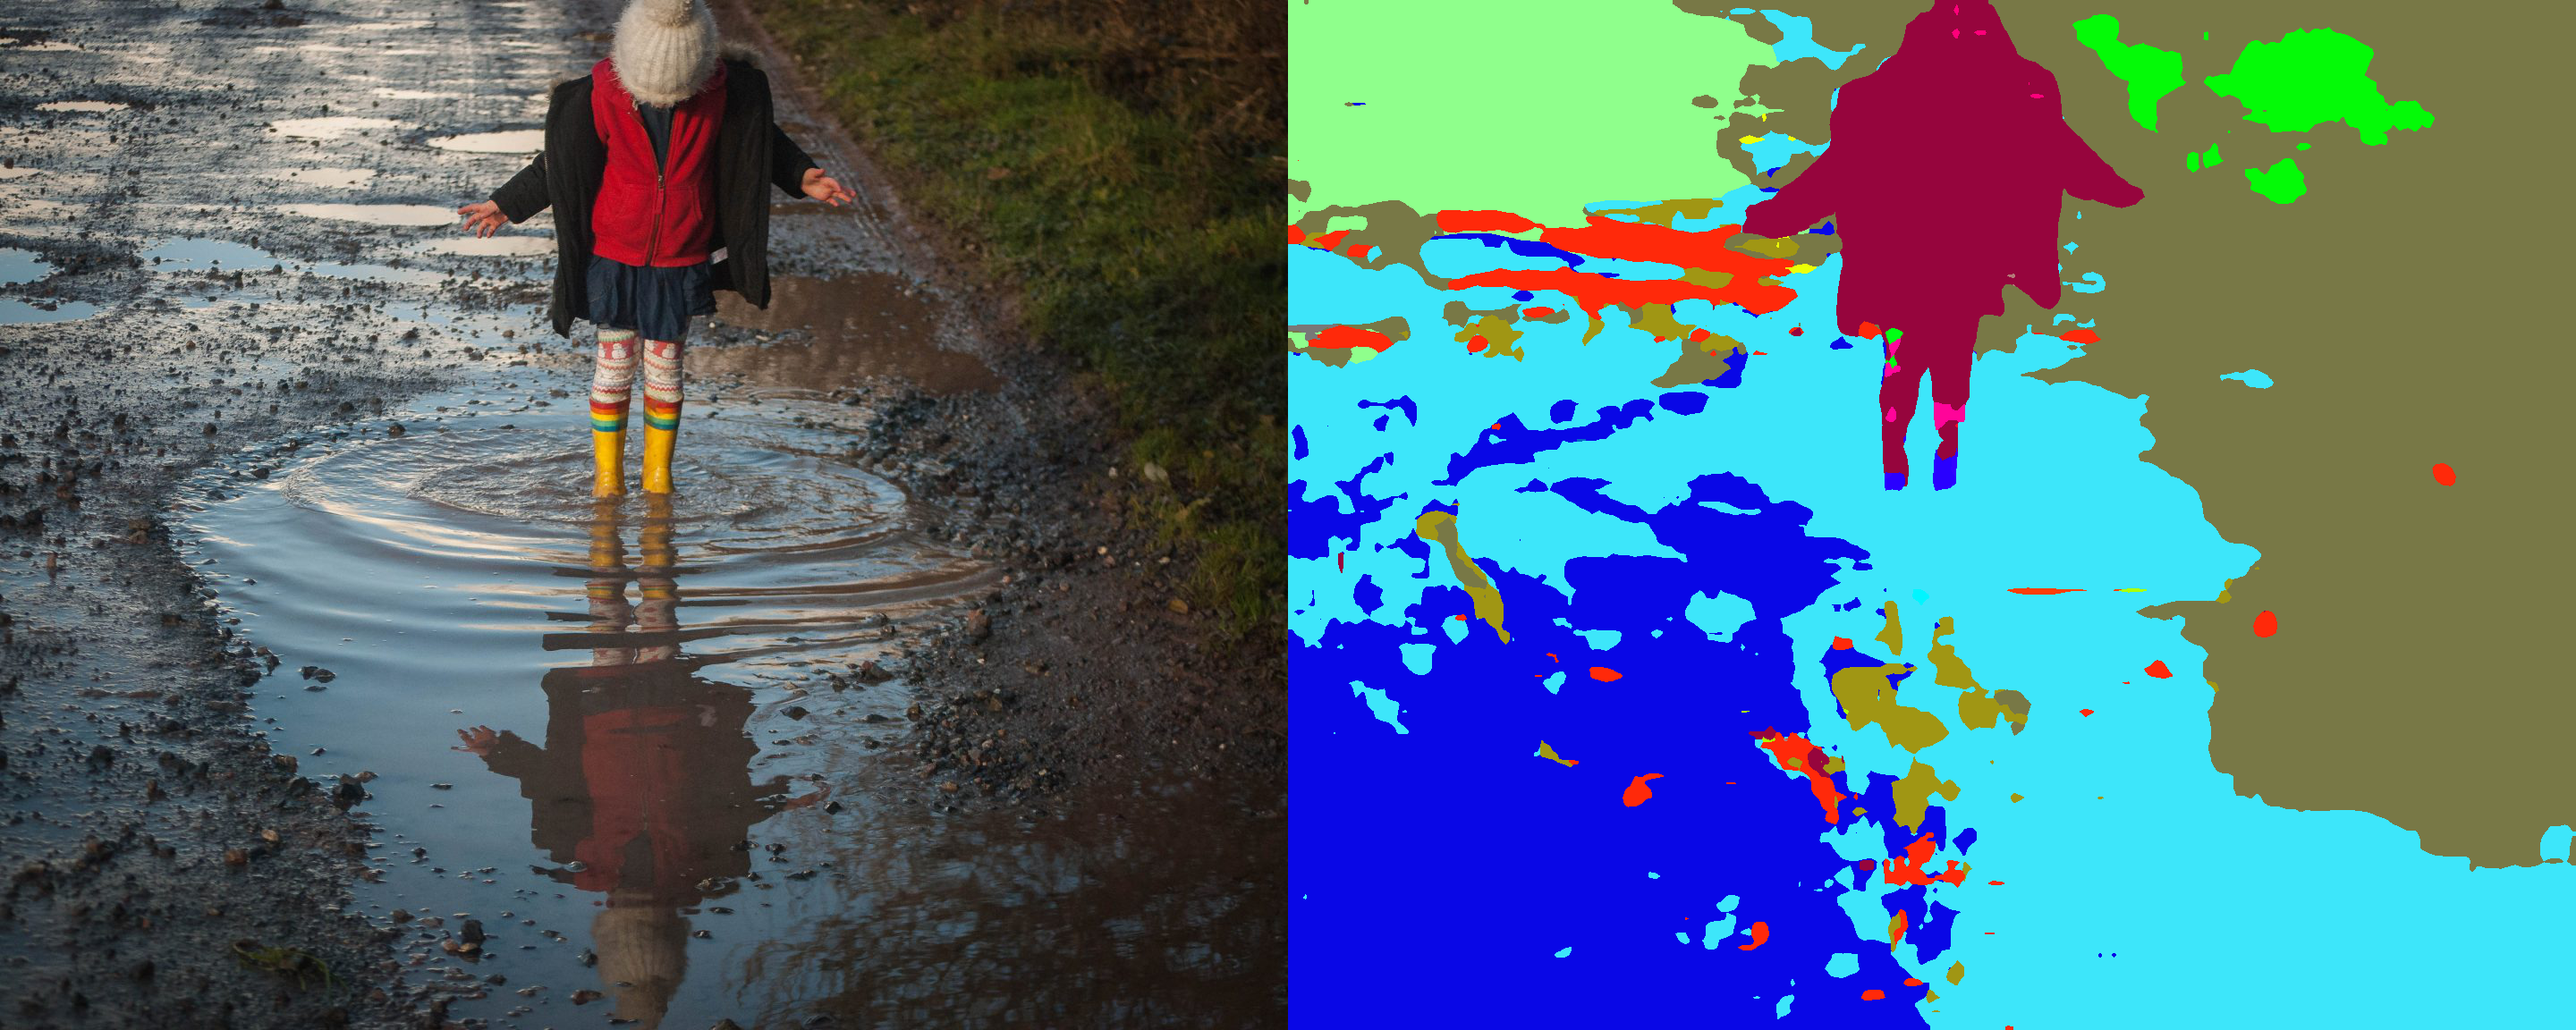
\includegraphics[width=\linewidth]{Figures/Formulation/image_seg_fail.png}
	\end{subfigure}
	
	
	\begin{subfigure}[b]{.8\linewidth}   
		\centering 
		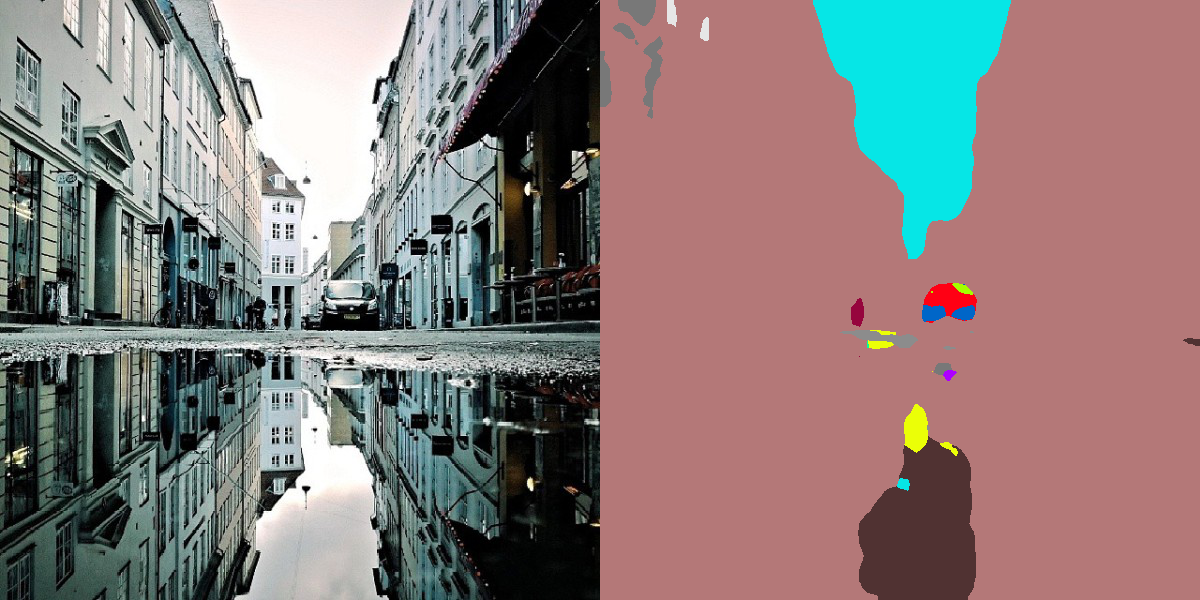
\includegraphics[width=\linewidth]{Figures/Formulation/image_seg_fail2.png}
	\end{subfigure}
	
	
	\begin{subfigure}[b]{.8\linewidth}   
		\centering 
		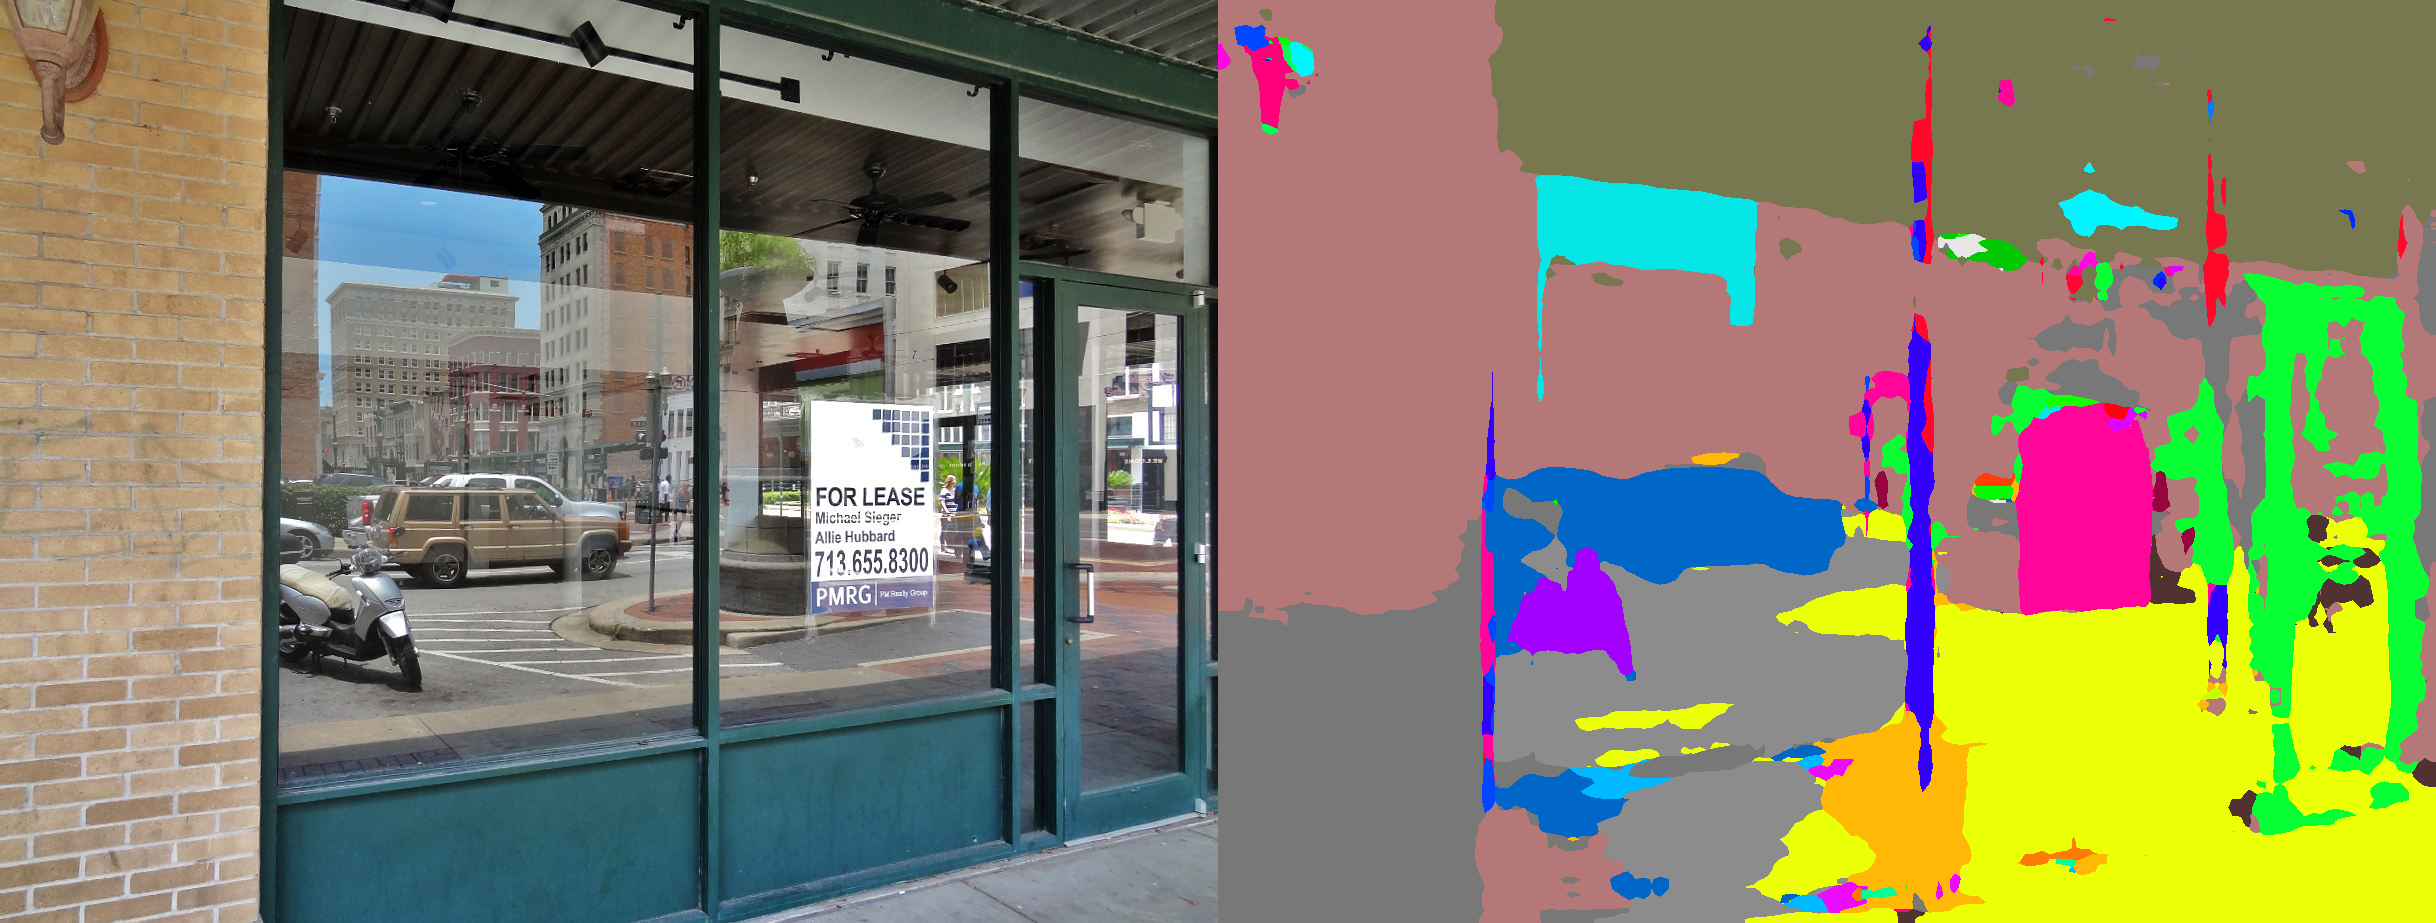
\includegraphics[width=\linewidth]{Figures/Formulation/image_seg_fail3.png}
	\end{subfigure}
	
	
	
	\caption[Reflection erroneous segmentations from RGB]{Segmentation results from \cite{zhou2018semantic} showing erroneous estimation on specular surfaces.}
	\label{fig:fail-seg}
\end{figure}

\subsection{Formulation}\label{form_pol}
With the objective of developing an algorithm relying on reflection to define urban scenes, it is necessary to formulate the problem. As mentioned before, we start from a statement: urban scenes are mostly subject to specular reflection. This phenomenon is even amplified when the weather conditions are unfavorable. Plus, although standard algorithms have acceptable performances in common environments, they tend to fail when they are in the presence of specular reflection, especially when observing puddles. Moreover, the methods are unhelped by the usual datasets since they generally do not contain any of these occurrences.




As shown in the figure \ref{fig:fail-seg}, algorithms that perform well in favorable cases tend to miss their estimate when they observe specularity. This kind of erroneous estimation can be problematic especially if an autonomous vehicle algorithm depends on these estimates.

However, it is necessary to bound the polarimetric images to obtain the desired effect: discriminate and simplify the problem.
Unprocessed, polarization images are not really usable. As described in the Section \ref{Polar_explain}, the images are sparse and not particularly descriptive. If the raw images are preserved, it is challenging to constrain the problem since the specularity is only defined by the pixel saturation. Although it is indeed characterized, it is necessary to transpose these images through the Stokes parameters to implicitly extract the informative part of the images. Consequently, and in order that the images are exploitable by a CNN, it is necessary to decide on an exploitable representation image.


\subsection{Image Representation}\label{rep_pol}

One critical point of machine understanding approaches is to have representative and understandable images. 
Image representation is omnipresent in the field of computer vision. On the other hand, it has become progressively transparent. The colorimetric images are subject to an image representation allowing to pass from the lowest level (raw) the Bayer matrix, to a composition in three channels, traditionally RGB.
Polarization is not exempt from this, however, since the modality is unconventional and not as widely used, it is necessary to define advantageous rules to the future processing pipeline.

Our goal is to have a reliable and representative image while making it deep learning-friendly. Thus, according to our problem the images must intrinsically represent polarization and by extension specularity while preserving differentiable textures allowing the network to learn. 
Starting from the raw images, we recover the informative part of the images by computing the Stokes parameters:

\begin{equation}
S = \begin{pmatrix}s_0\\s_1\\s_2\\s_3\end{pmatrix} = \begin{pmatrix}P_H + P_V\\ P_H - P_V\\ P_{45} - P_{135} \\ P_R - P_L\end{pmatrix} = \begin{pmatrix}P_0 + P_{90}\\ P_0 - P_{90}\\ P_{45} - P_{135} \\ 0\end{pmatrix},
\end{equation}

where $s_n$ is the $n^{th}$ Stokes parameter and $P_\Theta$ is the dense polatization image corresponding to the $\Theta$ angle oriented polarizer.
It is notable that the $P_\theta$ images must be dense and therefore that between the raw imagery and these, it may be necessary to interpolate the images between pixels to densify them. This will depend mainly on the image resolution of the camera.
Also, recall that in the absence of a quarter-wave plate, no circular polarization $s_3$ is acquired.
From these, it is possible to easily find the three strong descriptors of the polarization, the intensity $\iota$, the polarization angle $\alpha$ and the degree of polarization $\rho$:
\begin{equation}
\iota = \frac{P_0 + P_{45} + P_{90} + P_{135}}{2},
\end{equation}
\begin{equation}
\rho = \sqrt{\Bar{s_1}^2 + \Bar{s_2}^2},
\end{equation}
\begin{equation}
\alpha = \frac{1}{2}\textrm{tan}^{-1}(\frac{s_1}{s_2}),
\end{equation}

where $\bar{s_n}$ is the $n^{th}$ Stokes parameter normalized by $s_0$.

Although there are a multitude of possibilities to combine these three images, it is necessary to consider their nature to obtain a representative result.
While $\iota$ is the texture of the image, it is a standard grayscale image, $\alpha$ and $\rho$ are two complementary images respectively the angle of projected reflection and its "strength". It is then necessary to aggregate this information to maintain the integrity and especially the interest of the polarization. Thus, the raw concatenation would strongly reduce the interest of the imaging for PwSS applications.

Also, to avoid imposing a relearning of the organization of the pixels for the network, but also to benefit from the advantages of the transfer learning, it is necessary to move towards a three-channels structure.

\begin{figure}[h]
	\centering
	\begin{subfigure}{.4\textwidth}
		\centering
		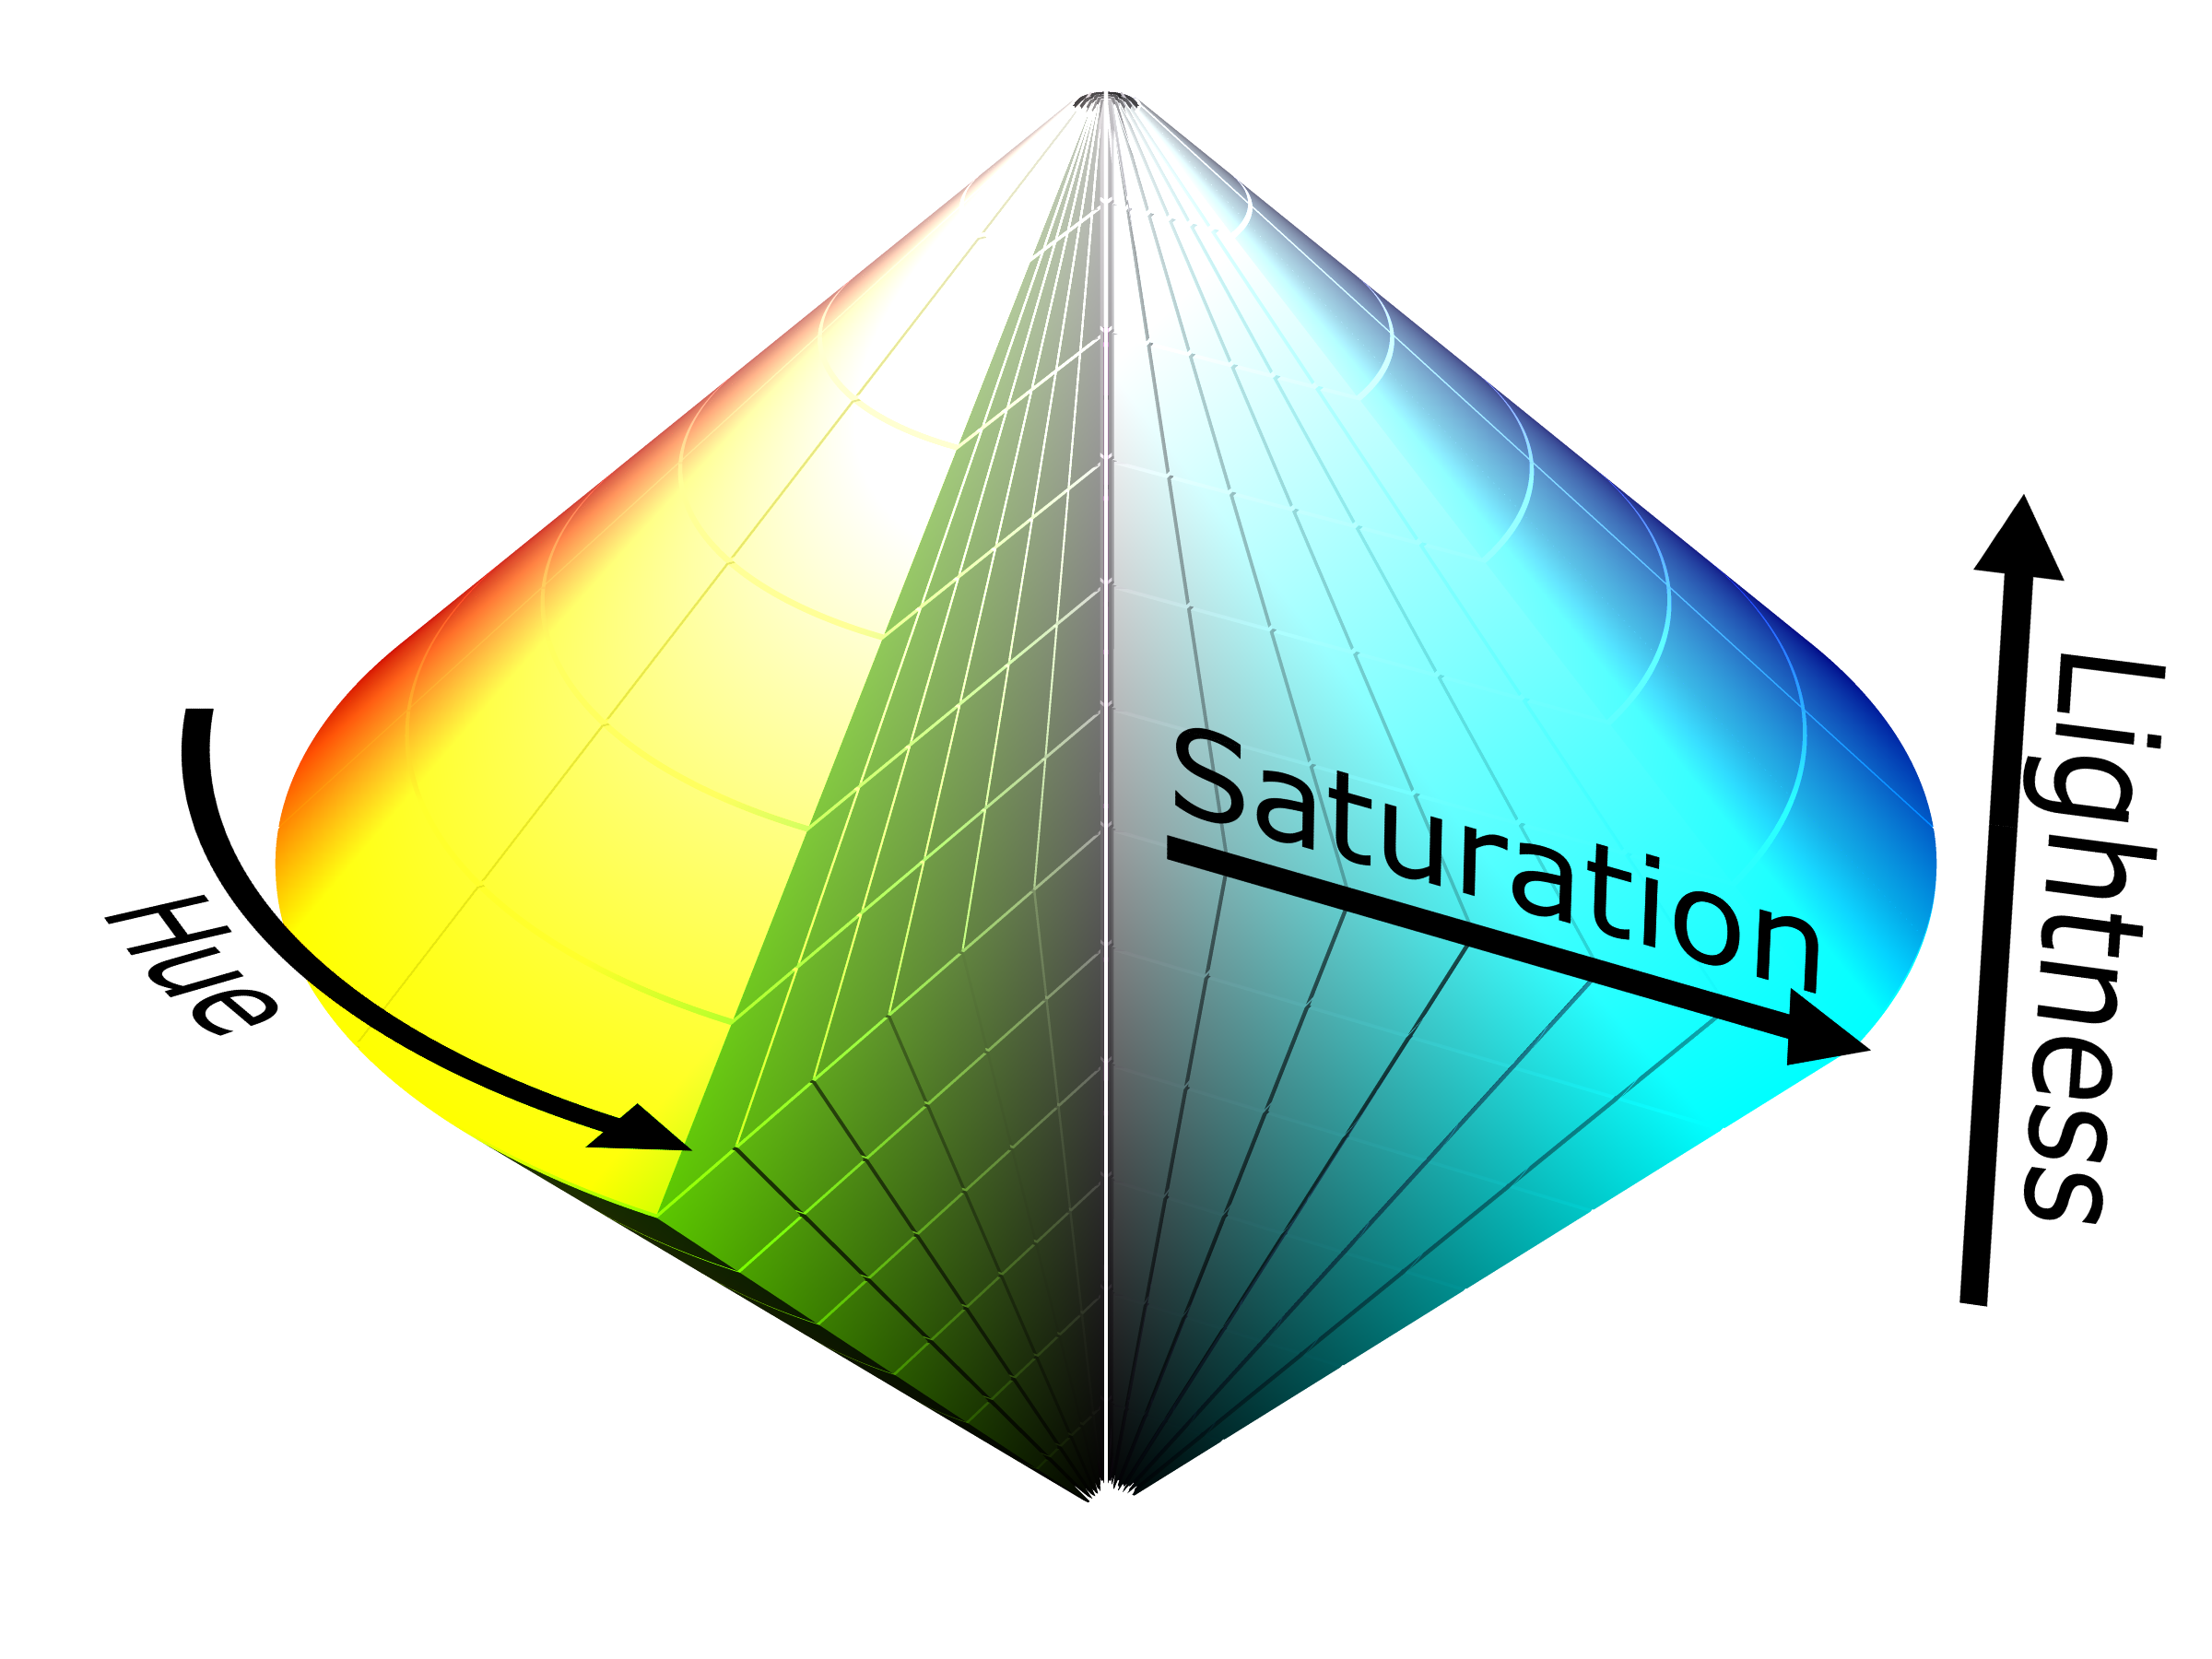
\includegraphics[width=\linewidth]{Figures/Representation/HSL_block.png}
	\end{subfigure}
	\begin{subfigure}{.4\textwidth}
		
		\centering
		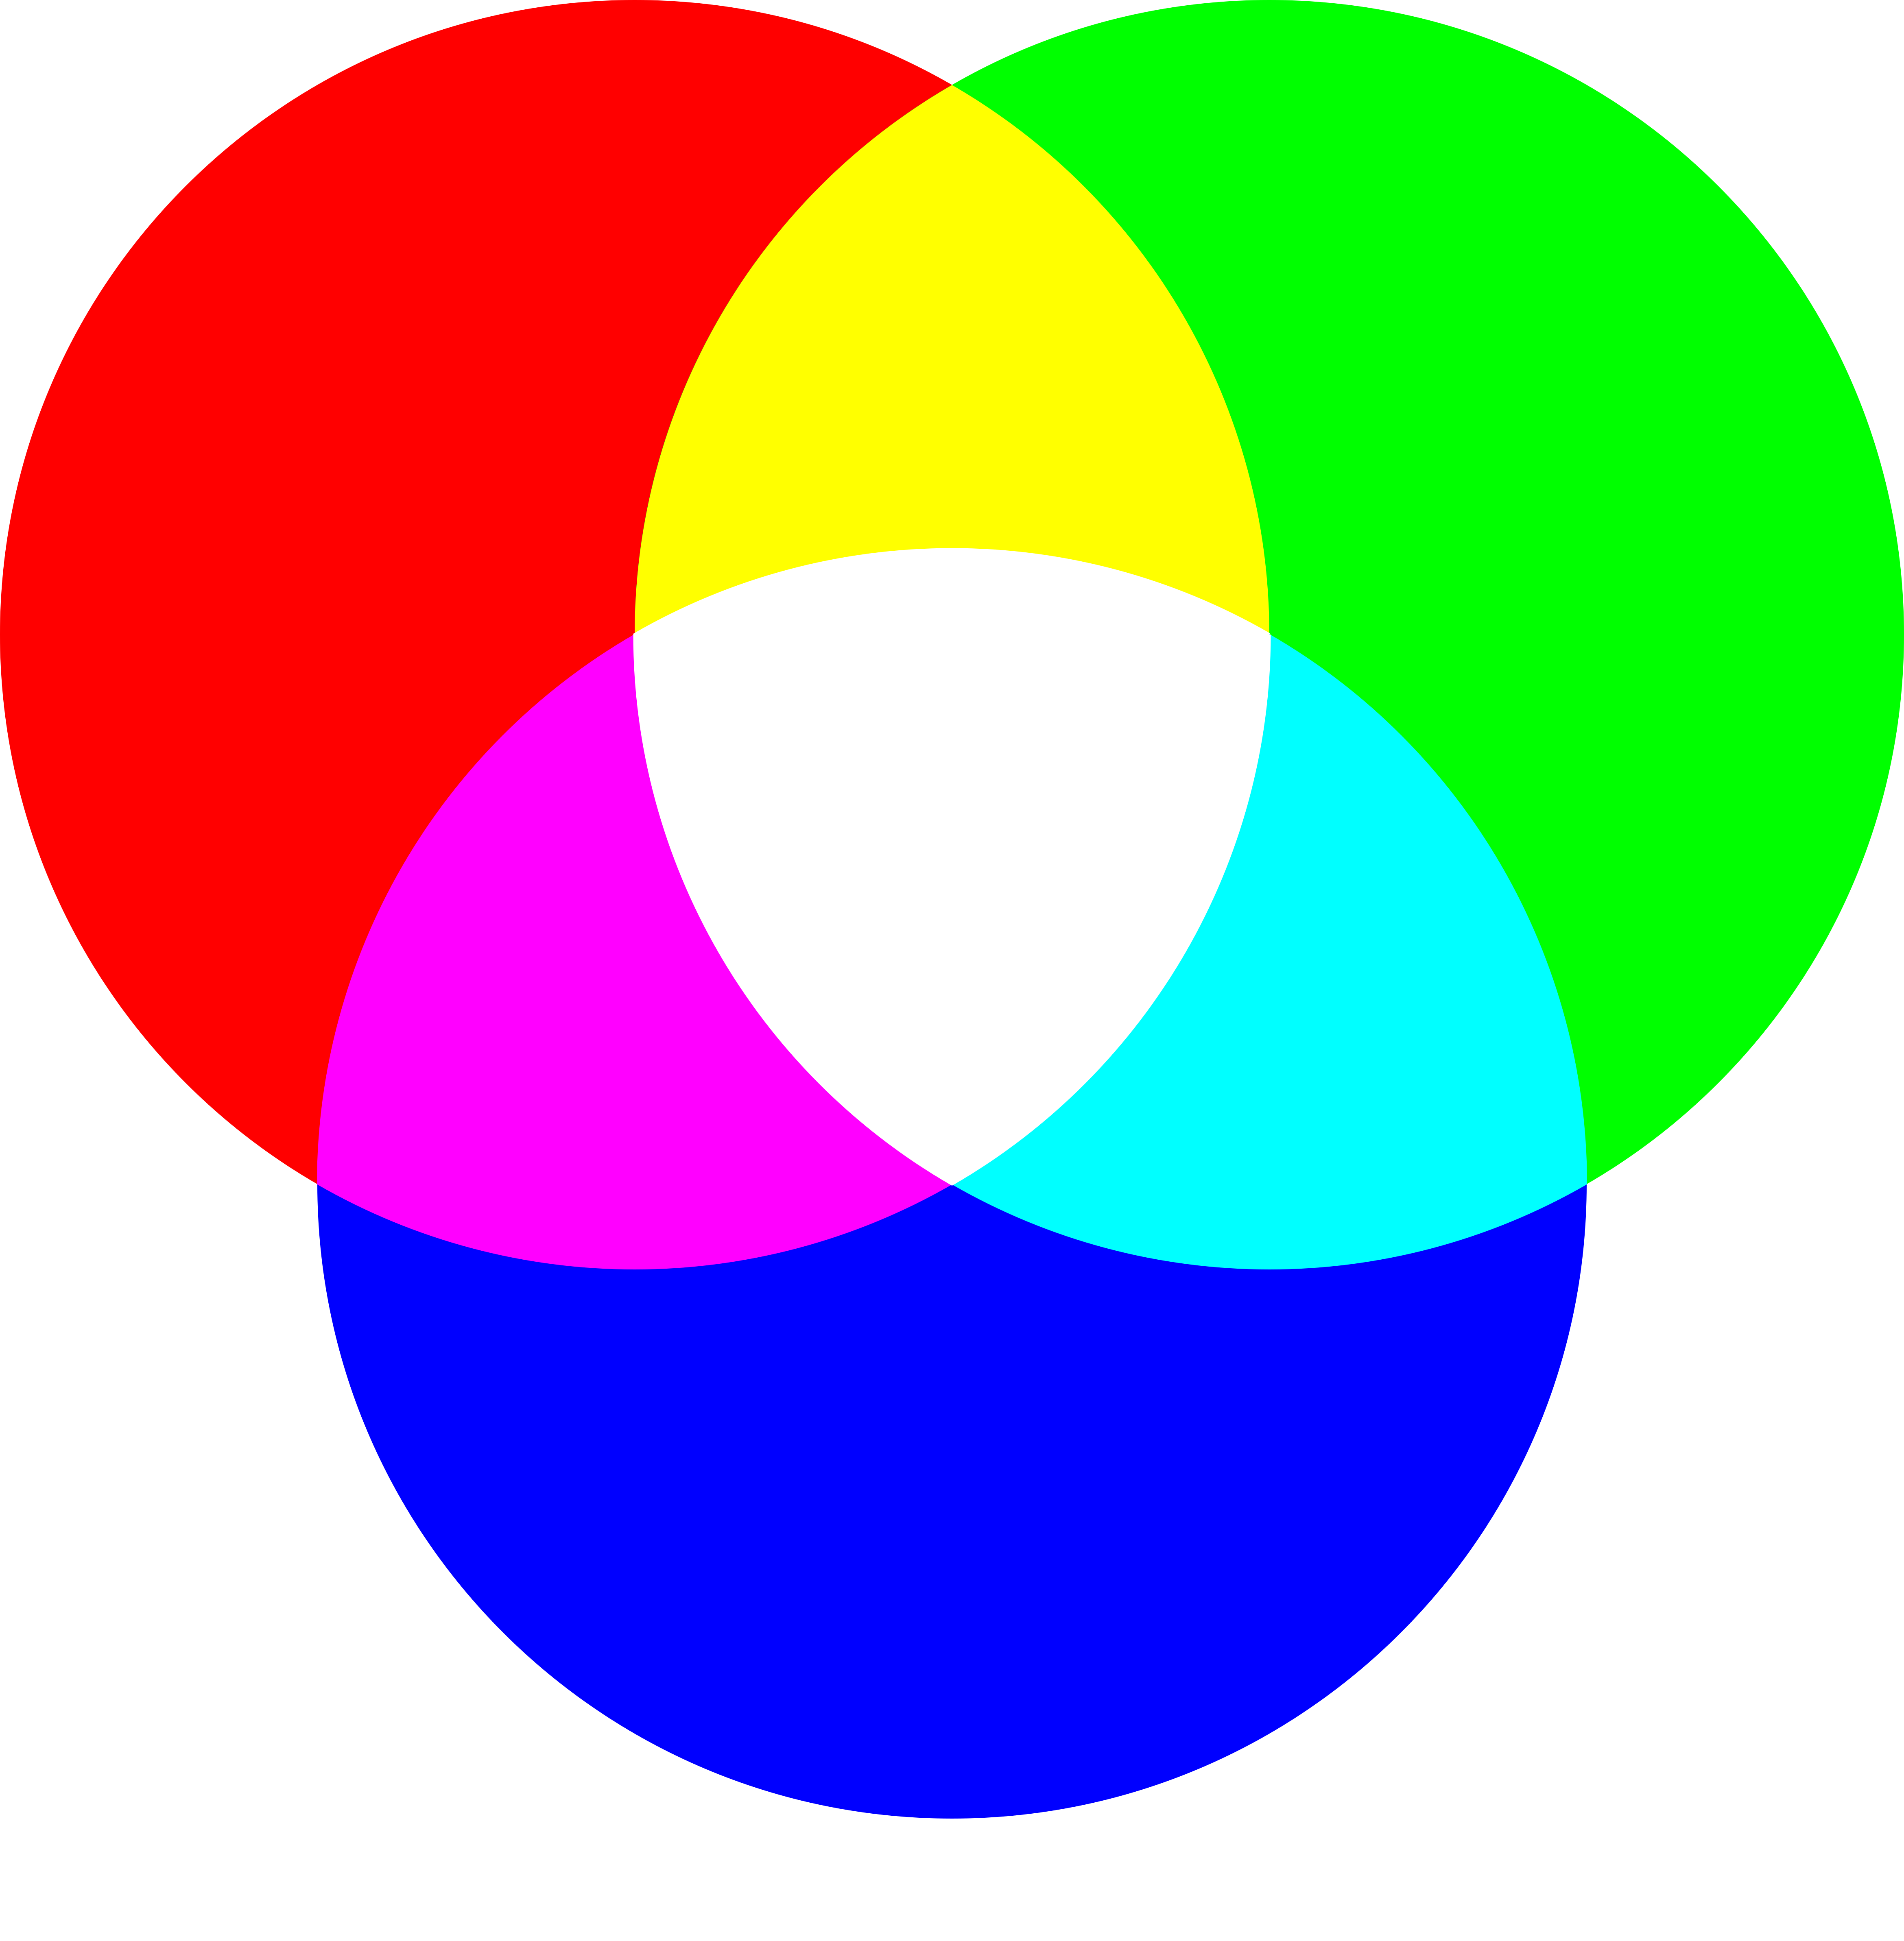
\includegraphics[width=.7\linewidth]{Figures/Representation/RGB_wheel.png}
	\end{subfigure}
	\caption{HSL and RGB color models.}
	\label{fig:hslrgb}
\end{figure}


In this context, we propose representing these images in three HSL channels as proposed by \cite{wolff1995polarization} that will finally be transposed in RGB color space\footnote{Converting toolbix available at: \url{https://github.com/BlanchonMarc/InterPol}}. Indeed, this intermediate format allows infusing particular properties to the image, while keeping a simple transposability from HSL to RGB. As shown in the Figure \ref{fig:hslrgb}, both modelization formats include a singular behaviour.

The RGB model is widely operated since it is direct and additive. In contrast, Hue Saturation and Luminance (HSL) is somewhat different due to its cylindrical and cyclic nature. This model enjoys many advantages, but the prominent attraction for polarimetry is that its channels are neither bounded nor processed in the same way. They are therefore independent but complementary for visual representation.
The key advantage of the HSL representation is its channel coding.Indeed, the three separate channels are quantized differently and allow a direct adaptation with the polarization.
Hue represent a cyclic value between 0 and 360 which comfortably accommodates a $2\pi$-periodic value and thus the polarization angle.
The saturation represents the intensity of the color indicated by the Hue. It is a percentile value that allows an analogy with the degree of polarization. The correspondence between the color and its intensity of this mode is convenient to use with polarization and the proper properties of $\alpha$ and $\rho$.
Finally, L, the luminance, can easily accommodate the intensity value $\iota$ since its utility is very similar to the encoding of a texture.
In conclusion, the polarimetric images will be mapped as:

\begin{equation}\label{eq:hsl}
H \longrightarrow 2*\alpha,  \quad S \longrightarrow \rho, \quad L \longrightarrow \frac{\iota}{255}.
\end{equation}

\begin{figure}[h]
	\centering
	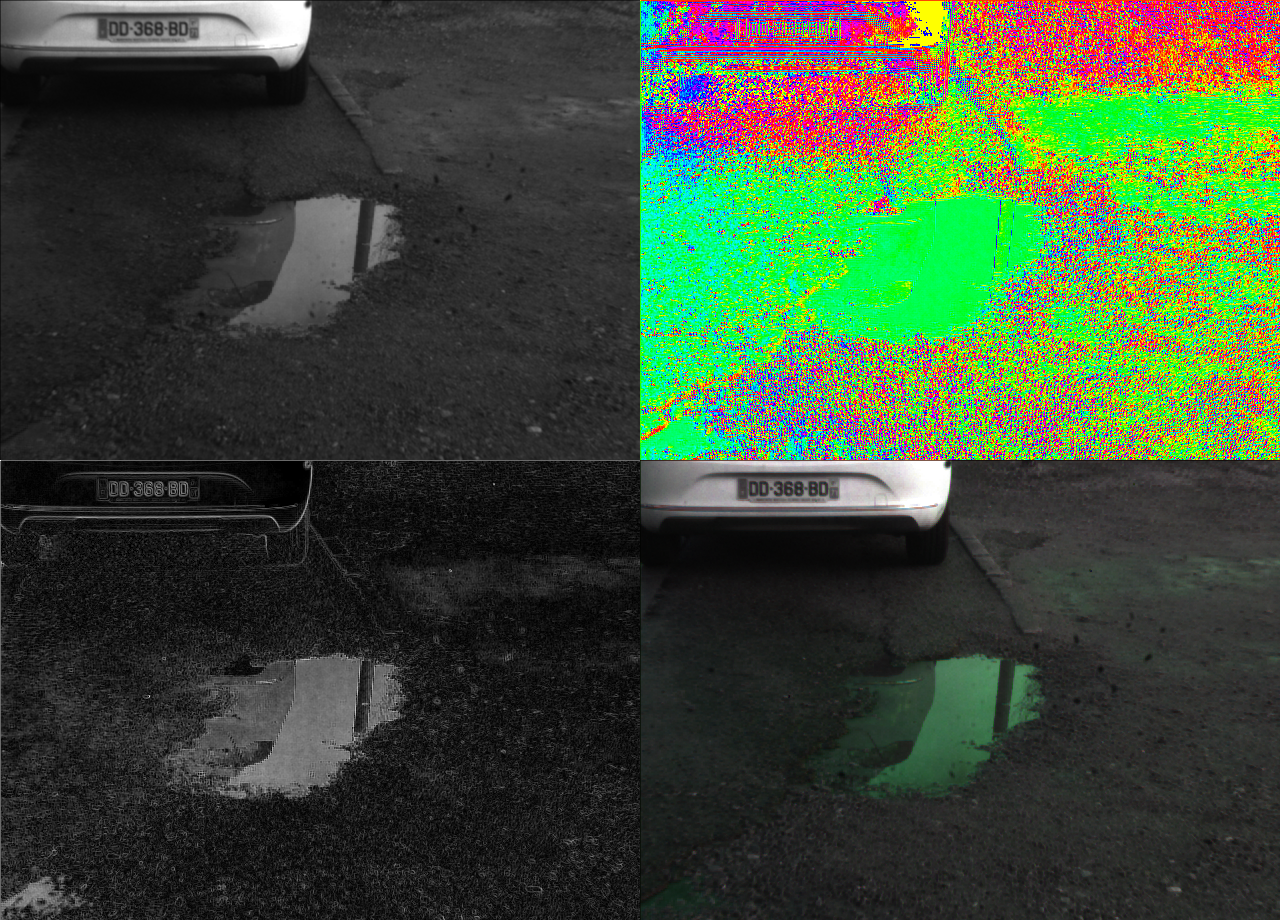
\includegraphics[width=0.8\linewidth]{Figures/Representation/4im}
	\caption[HSL representation of polarization.]{HSL representation of polarization. At the top left is the intensity $\iota$, then at the top left the polarization angle $\alpha$. At the bottom left is the polarization degree $\rho$ and at the right is the combination of the three informative images in HSL format and the equation \ref{eq:hsl}.}
	\label{fig:4im}
\end{figure}


As shown in the Figure \ref{fig:4im}, it is remarkable that the images are peculiar and that their hue is unnatural. Indeed, the texture is present but colors are affected according to the $alpha$ orientation. Also, the intensity of the color is decided by $\rho$. In the end, the more a zone is colored, the more it is polarized. And according to the color, the various angles are observable in a transparent way.

After this representation, a three-channel image is obtained which could be used as input for a DCNN. 
Regrettably, remarkably few models are trained with HSL-mode data, and the convention is until now RGB for the training task. 
Rather than having to end-to-end train a network by training the data encoding, it is more convenient to use RGB. Indeed, this will allow using pre-trained networks and thus to benefit from approved transfer learning methods.
As follows, the choice is considered to transpose the HSL images in RGB while keeping the particular display properties following the system:

\begin{equation}
	C = (1 - |2L - 1|) \times S,
\end{equation}
\begin{equation}
	X = C \times (1 - \Big| \frac{H}{60^\circ} \mod 2 - 1 \Big| ),
\end{equation}
\begin{equation}
	m = L - \frac{C}{2},
\end{equation}
\begin{equation}
	(R^\prime,G^\prime,B^\prime) = 
	\begin{cases}
		(C,X,0) & \mbox{, }0^\circ \leq H < 60^\circ  \\
		(X,C,0) & \mbox{, }60^\circ \leq H < 120^\circ \\
		(0,C,X) & \mbox{, }120^\circ \leq H < 180^\circ \\
		(0,X,C) & \mbox{, }180^\circ \leq H < 240^\circ \\
		(X,0,C) & \mbox{, }240^\circ \leq H < 300^\circ \\
		(C,0,X) & \mbox{, }300^\circ \leq H < 360^\circ  
    \end{cases},
\end{equation}
\begin{equation}
	(R,G,B) = \Big( (R^\prime+m)\times 255, (G^\prime+m)\times 255,(B^\prime+m)\times 255 \Big).
\end{equation}

After all these transformations to interpret the polarization, a polarimetric RGB-coded image is obtained.


\subsection{Dataset}\label{data_pol}

The dataset is a critical element when using machine learning algorithms. The scientific community agrees it is one of the most crucial points if not the most important.
Conventionally, since DL-based methods are greedy, the more data the better. This is accommodating when using a widespread and easily acquired modality. On the other hand, when addressing non-conventional modalities, the major obstacle for the community is the need for a massive amount of data.

Our approach is somewhat alternative although also constrained by modality. The idea is to obtain viable results with the limited data available.
First, it is necessary to acquire data in urban areas and under adverse conditions.

We constituted Polabot\footnote{Available at: \url{http://vibot.cnrs.fr/polabot.html}}, a multimodal oriented dataset composed of 3 synchronized modalities: polarization, colorimetry and near infrared, acquired with the cameras referenced in Table \ref{carac}. 
As a final image collection, it is composed of 178 multimodal aligned, synchronized and annotated urban scene images with eight unique classes: unlabeled, sky, water, windows, road, car, building and none. Unlabeled corresponding to segmentation errors during manual annotation and none being the areas defined as irrelevant for our application. The different scenes propose several complex scenarios composed of puddles or buildings' windows which are often incorrectly estimated in usual methods.
Since this collection is very restricted and insufficient to train a sustainable model, the augmentation presented in Section \ref{aug_4} represent a required requirement.

Yet, the acquisition of this dataset involves two major challenges prior to the augmentation: the synchronization of images from several sources and their alignment which will be respectively presented in \ref{sync} and \ref{align}.

\subsubsection{Synchronization}\label{sync}

One of the problems of acquisition of any multimodal and multifocal system remains the synchronization of images. To be specific, desynchronization can cause a detrimental effect when images are captured at high speed. A shift and the images do not exhibit sufficient correlation due to the distance traveled between two image triggers.
In our case, the de-synchronization is negative for this distance problem but also specifically for the cross-modality performance comparison. Indeed, as previously stated, this dataset allows us to train networks but also and especially to have a point of comparison to determine the advantage of a modality over another for our application.
To prevent desynchronization errors, we have developed a rule-based system\footnote{Available at: \url{https://github.com/BlanchonMarc/Ros_AcquisitionFromTopics}} to ensure the smallest possible cross-modality shift.

\begin{figure}[h]
	\centering
	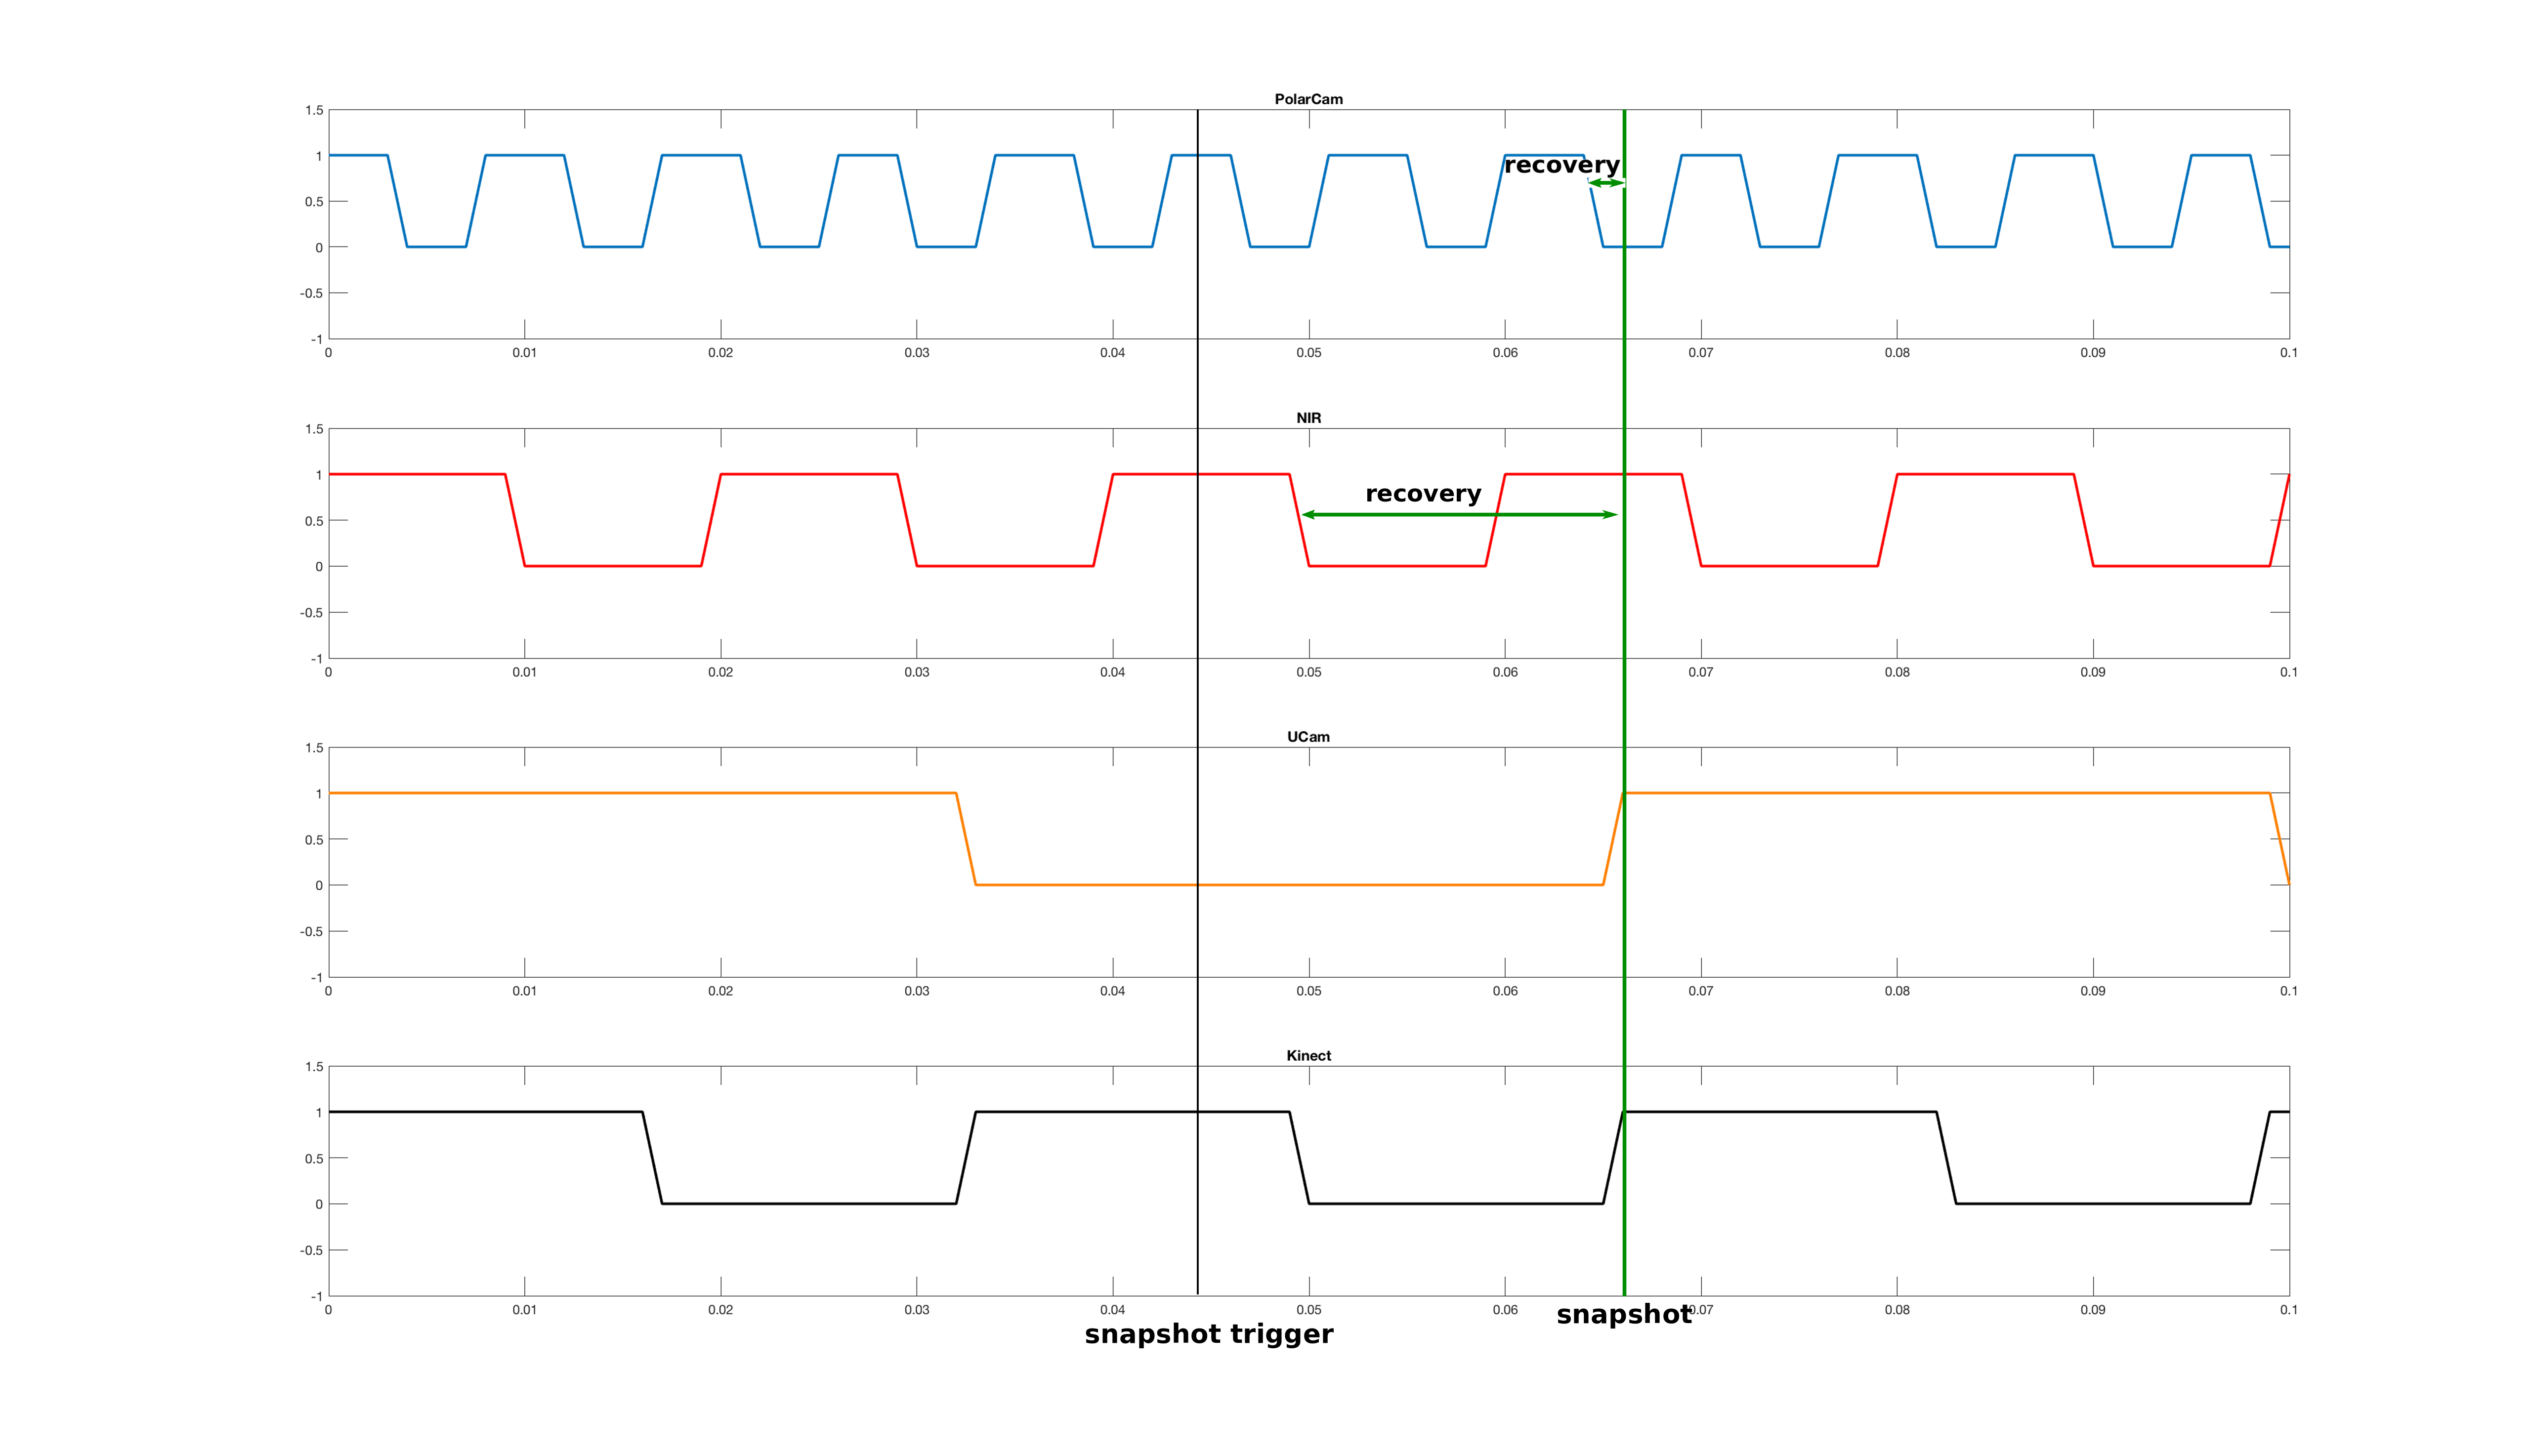
\includegraphics[width=0.8\linewidth]{Figures/Dataset/freqgraphnew}
	\caption{Recovery strategy-based synchronization.}
	\label{fig:freqgraphnew}
\end{figure}


The principle is to consider snapshot trigger signal. The cameras have a discontinuous image stream and this can be represented by square signals. As shown in the Figure \ref{freqgraphnew}, each rising edge corresponds to an image trigger (replacement of the previous image). The strategy is simple, at each artificial trigger, it is necessary to wait for the following acquisition of the slowest camera and then use a recovery strategy.

In conclusion, this simple rule-based strategy allows to drastically reduce the problems related to desynchronization and therefore to eliminate artifacts such as shift, motion blur or displacement between images.

\subsubsection{Multimodal Alignment}\label{align}

Image alignment represent a well-known field. Very well defined, this problem is for the most part solved. However, when addressing the idea of multimodal alignment, known methods can be inefficient, especially when the images to be aligned are non-interpolatable.
This is indeed the case handled in this section. The concept is to efficiently align an RGB image with a polarimetric image. It is significant to experience a precise framing since the correspondence at pixel level must be exact. Thus, a valid comparison can be performed between the segmentation results from independent networks addressed on different modalities.

\textbf{Homography-based.} Homography \cite{artin1957geometric,baer2005linear} is one of the most popular methods to estimate the displacement between two images. Assuming that two images are on the same plane in space then they are linked by the homography. 
There is on top an underlying assumption that the two images must be in the same feature space. This is not the case between colorimetric and polarimetric imaging. However, it is completely possible to find a common space in grayscale intensity.
\begin{figure}[h]
	\centering
	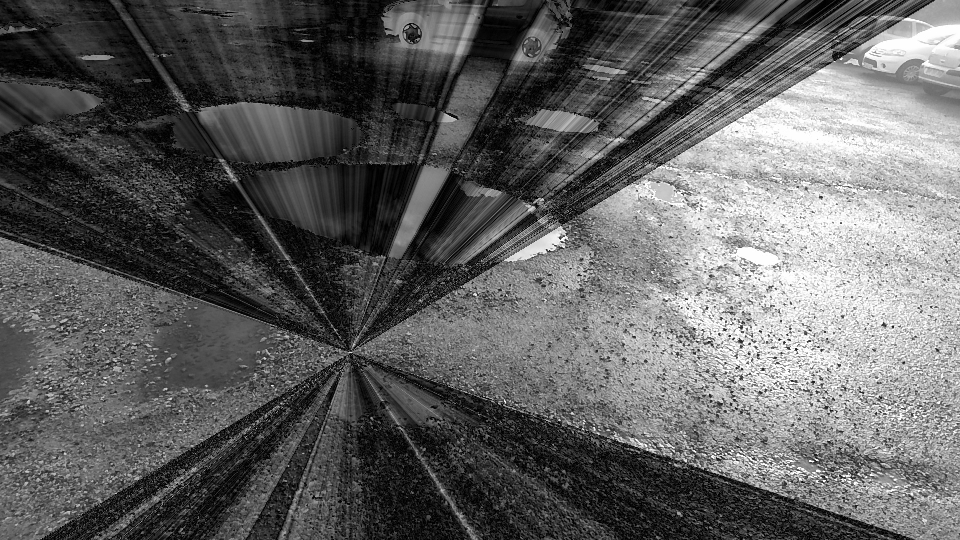
\includegraphics[width=0.8\linewidth]{Figures/Dataset/VISWarp}
	\caption{Innacurate alignment through homography estimation.}
	\label{fig:viswarp}
\end{figure}
Then, just find and map the corresponding feature points on each image and deduce the transformation. The result is $R$ and $t$, the rotation matrix and the translation vector that allow to transform an image to align it with another one. 
This process is remarkably rapid and practical, but it suffers some disadvantages which are induced by the hypotheses stated above. Since the polarization is not interpolable, it is impossible without extra-computation to preserve the properties of the image. Therefore, it is mandatory to move only the colorimetric image and map it to the polarization. Secondly, it should be noted that the polarimetric and colorimetric intensities are supposed to be theoretically almost identical, but in reality, the inconsistencies between them lead to erroneous estimates. In the Figure \ref{fig:viswarp}, a case of alignment of RGB to inaccurate polarization is shown. 




Since there are inconsistencies between the spaces, it is then necessary to go one step further to allow an accurate alignment.

\textbf{Homography-initialized dense alignment.} Since a simple transformation through homography proves to be inefficient due to the nature of the images, it is possible to perform a dense alignment to refine it.

Directly inspired by image-based visual servoing methods, the proposed concept\footnote{Available at: \url{https://github.com/BlanchonMarc/process-vibotorch} } allows to refine the parameters $R$ and $t$ itteratively. 
Starting from the reference polarimetric image $I^*$ and the colorimetric image $I_c$, an error $\epsilon$ is computed such that:

\begin{equation}
\epsilon = I^* - I_c.
\end{equation}

It is then possible to determine an interraction matrix $L$  \cite{chaumette2006visual} following: 

\begin{equation}
L = \begin{bmatrix}
-1/Z       & 0 & \Delta_{x}/Z & \Delta_{x}\Delta_{y} & -(1+\Delta_{x}^2) & \Delta_{y}  \\
0      & -1/Z &  \Delta_{y}/Z & 1 +  \Delta_{y}^2 & -\Delta_{x}\Delta_{y} & -\Delta_{x} 

\end{bmatrix},
\end{equation}

with $Z$ the distance between the plane and the camera, $\Delta_x $ the gradient along x and $\Delta_y $ along y.
From the pseudo inverse of $L$ and $\epsilon$ is derived the velocity vector such that: 

\begin{equation}
v = -\lambda L^+ \epsilon,
\end{equation}

with $\lambda$ a scalar. Thanks to the velocity vector, the Lie algebra and the exponential map \cite{reutenauer2003free}, the increments $\hat{R}$ and $\hat{t}$ can be evaluated according to: 

\begin{equation}
\hat{R}, \hat{t} = \textrm{exponential map}(v).
\end{equation}

Finally, using the pose increments and an initial homography $H$, a new transformation matrix $\hat{H}$ can be estimated:

\begin{equation}
\hat{H} = K \times \bigg[ (R\hat{R}) + (t + \hat{t}) \times \frac{n^T}{d} \bigg] \times K^{-1},
\end{equation}

with $K$ the intrinsic parameters of the camera acquiring the image $I_c$.

\begin{figure}[h]
	\centering
	\begin{subfigure}{.4\textwidth}
		\centering
		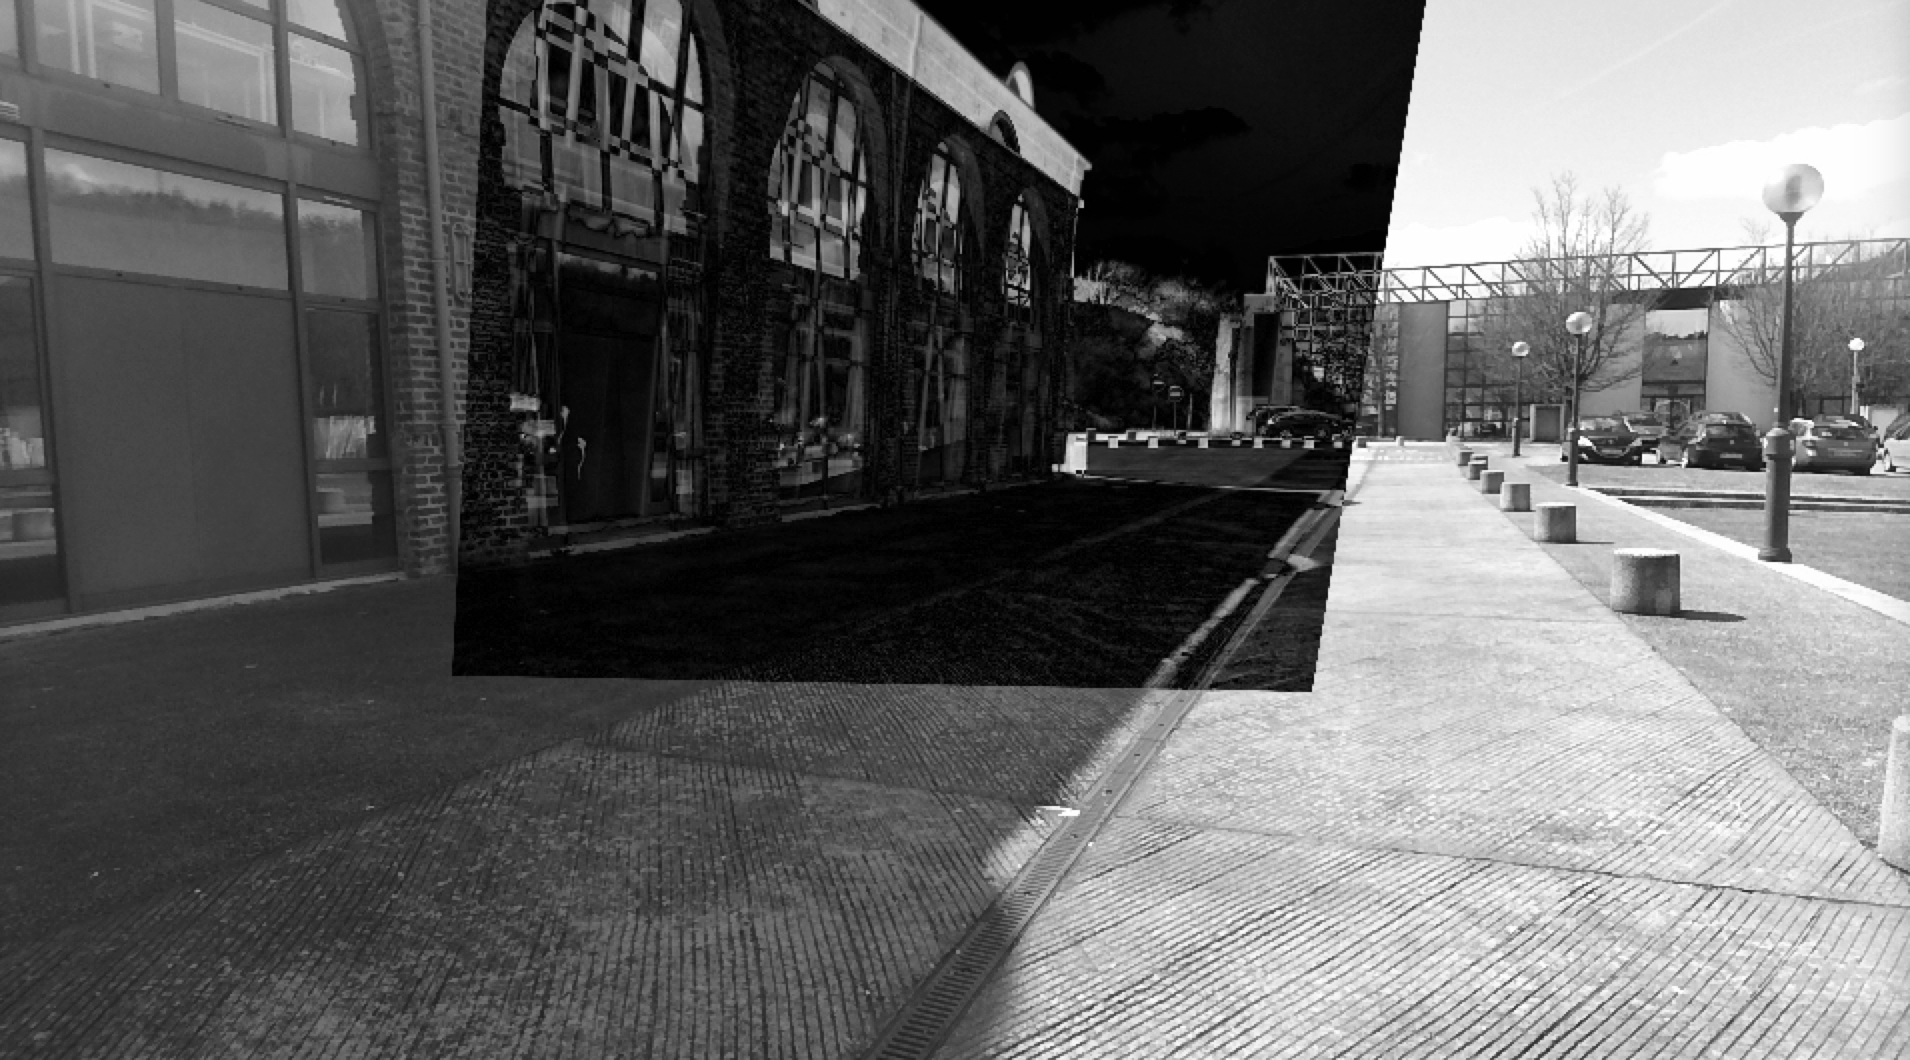
\includegraphics[width=\linewidth]{Figures/Dataset/beforealign.png}
	\end{subfigure}
	\begin{subfigure}{.4\textwidth}
		
		\centering
		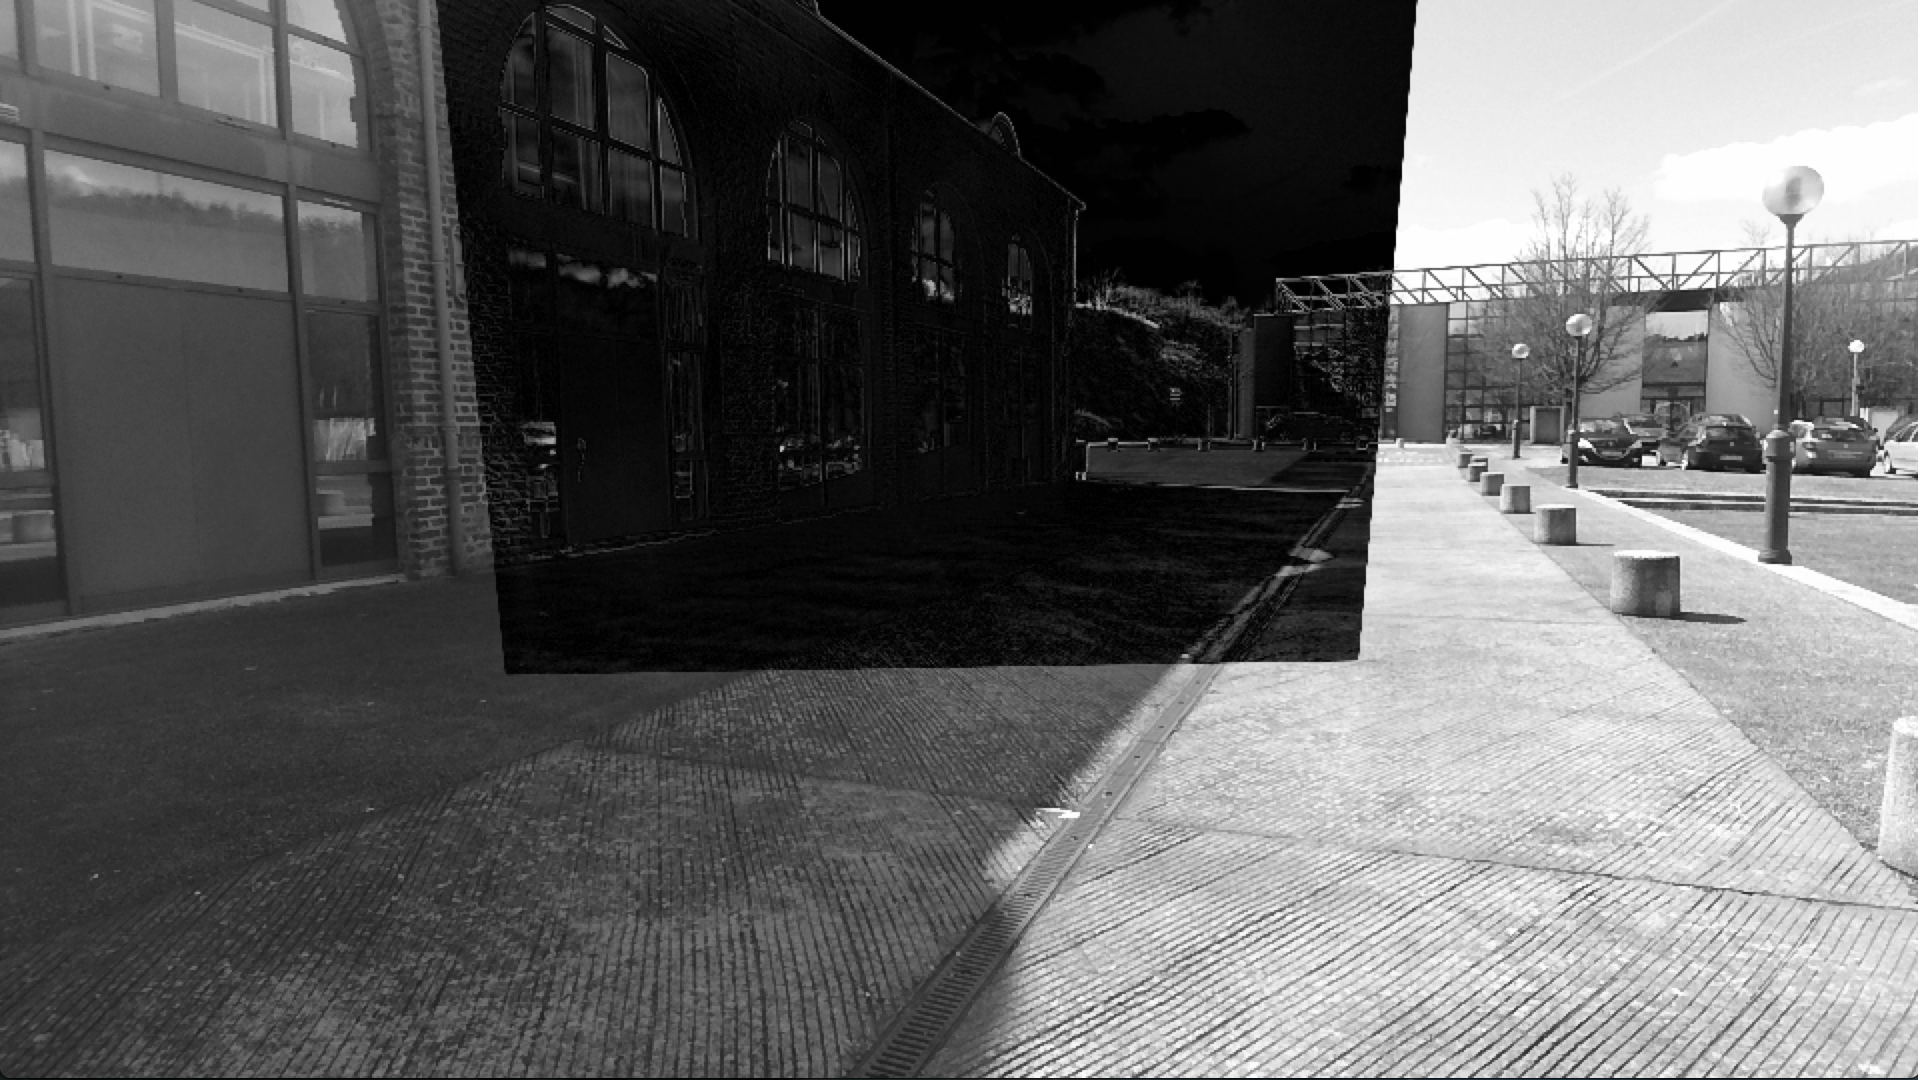
\includegraphics[width=\linewidth]{Figures/Dataset/afteralign.png}
	\end{subfigure}
	\caption{Before and after dense alignment between polarimetric and RGB intensity images.}
	\label{fig:beforeafteralign}
\end{figure}


It is then possible to minimize the function through an iterative process or, in our case, to define an error target $\epsilon$. Indeed, since the starting hypothesis has invalidated the possibility of photometrically comparing the intensity images, we must empirically set an error threshold that will satisfy the alignment needs.
In addition, there is the parameter $Z$ that must be estimated or evaluated using a grid search approach. Finally, as shown in the Figure \ref{fig:beforeafteralign}, dense alignment seems to represent a viable solution. It is however important to mention the computational requirements are high and that this kind of process is heavy. Despite its efficiency, it is a matter of obtaining a tradeoff between a potentially precise alignment and a computation time consistent with the application.
In our dataset construction application, there is no online alignment which does not subject our pipeline to the slowness induced by this kind of process.

\section{Augmentation}\label{aug_4}

Augmentation has a major interest when dealing with a limited amount of data. This procedure allows to generalize the DCNN models and avoid overfitting \cite{DBLP:journals/corr/abs-1712-04621}.
However, this process has been principally designed to increase the population of interpolable modalities, but polarization cannot straightforwardly benefit from it by its nature.

Since the information acquired through a polarimetric sensor is intrinsically dependent on its pose, seeking a transformation without adaptation is invalid.
For these reasons, we have explored the augmentation operations applicable to polarization under any conditions.
Thus, we have estimated the two simple adaptable operations are the rotation and the flipping respectively described in \ref{rot} and \ref{syn}.
Finally, \ref{fin_proc} will be dedicated to the final reproducible procedure to multiply the polarimetric images.

\subsection{Rotation}\label{rot}

Rotation remain a very common operation to increase the number of images in a dataset. In practice it is enough to apply a rotation to the image and a new one is obtained. However, since the polarization information is relative to the camera pose, it is necessary to modify the operation.

The prerequisite for augmentation is to create new realistic images. If we transpose an image rotation to the sensor point of view, this procedure is equivalent to rotating the camera. 
This is where the constraint to polarimetry comes from, since pivoting the sensor means changing the camera pose.
Thus, altering the orientation of the camera changes the organization of the camera's pixel grid as shown in Figure \ref{rottheo}. And the objective is to reorganize these pixels so that the polarization angle regains its physical integrity.

\begin{figure}[h]
	\vspace{0.3cm}
	\centering
	\usetikzlibrary{patterns} % la librairie qui permet de remplir avec des motifs, cf le manuel : https://tex.stackexchange.com/questions/29808/can-i-control-the-density-of-a-pattern-in-tikz

% Pour personnaliser éventuellement les hachures : https://tex.stackexchange.com/questions/29808/can-i-control-the-density-of-a-pattern-in-tikz


% Autre fonction utile : la fonction clip, qui permet de découper une partie de dessin selon une géométrie
%
%
%INCLUDE ONCE

\tikzset{
    hatch distance/.store in=\hatchdistance,
    hatch distance=10pt,
    hatch thickness/.store in=\hatchthickness,
    hatch thickness=0.3pt
}

\makeatletter
\pgfdeclarepatternformonly[\hatchdistance,\hatchthickness]{northeast}
{\pgfqpoint{0pt}{0pt}}
{\pgfqpoint{\hatchdistance}{\hatchdistance}}
{\pgfpoint{\hatchdistance-1pt}{\hatchdistance-1pt}}%
{
    \pgfsetcolor{\tikz@pattern@color}
    \pgfsetlinewidth{\hatchthickness}
    \pgfpathmoveto{\pgfqpoint{0pt}{0pt}}
    \pgfpathlineto{\pgfqpoint{\hatchdistance}{\hatchdistance}}
    \pgfusepath{stroke}
}

\pgfdeclarepatternformonly[\hatchdistance,\hatchthickness]{northwest}
{\pgfqpoint{0pt}{0pt}}
{\pgfqpoint{\hatchdistance}{\hatchdistance}}
{\pgfpoint{\hatchdistance-1pt}{\hatchdistance-1pt}}%
{
    \pgfsetcolor{\tikz@pattern@color}
    \pgfsetlinewidth{\hatchthickness}
    \pgfpathmoveto{\pgfqpoint{\hatchdistance}{0pt}}
    \pgfpathlineto{\pgfqpoint{0pt}{\hatchdistance}}
    \pgfusepath{stroke}
}

\pgfdeclarepatternformonly[\hatchdistance,\hatchthickness]{horizontal}
{\pgfqpoint{0pt}{0pt}}
{\pgfqpoint{\hatchdistance}{\hatchdistance}}
{\pgfpoint{\hatchdistance-1pt}{\hatchdistance-1pt}}%
{
    \pgfsetcolor{\tikz@pattern@color}
    \pgfsetlinewidth{\hatchthickness}
    \pgfpathmoveto{\pgfqpoint{0pt}{0pt}}
    \pgfpathlineto{\pgfqpoint{\hatchdistance}{0pt}}
    \pgfusepath{stroke}
}

\pgfdeclarepatternformonly[\hatchdistance,\hatchthickness]{vertical}
{\pgfqpoint{0pt}{0pt}}
{\pgfqpoint{\hatchdistance}{\hatchdistance}}
{\pgfpoint{\hatchdistance-1pt}{\hatchdistance-1pt}}%
{
    \pgfsetcolor{\tikz@pattern@color}
    \pgfsetlinewidth{\hatchthickness}
    \pgfpathmoveto{\pgfqpoint{0pt}{0pt}}
    \pgfpathlineto{\pgfqpoint{0pt}{\hatchdistance}}
    \pgfusepath{stroke}
}
\makeatother


\begin{center}
\resizebox{\linewidth}{!}{
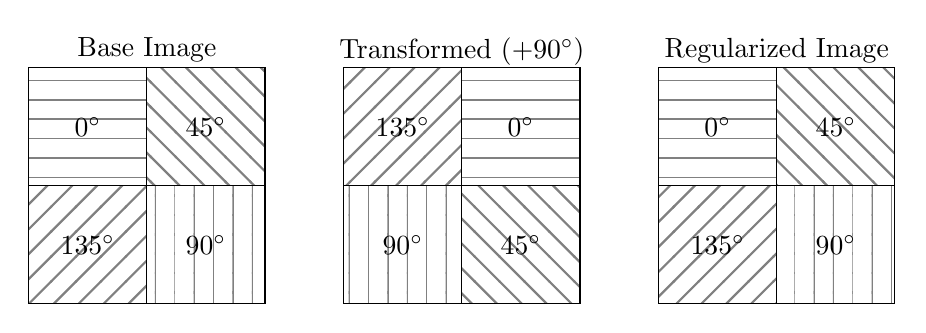
\begin{tikzpicture}

\draw[pattern=horizontal,pattern color=gray,hatch distance=8pt, hatch thickness = 0.8pt]  (0,1.5) rectangle (1.5,3)node[midway]{$0^\circ$}; % texte avec fond
 \draw[pattern=northwest,pattern color=gray,hatch distance=10pt, hatch thickness = 0.8pt] (1.5,1.5) rectangle (3,3) node[midway]{$45^\circ$};
 \draw[pattern=vertical,pattern color=gray,hatch distance=8pt, hatch thickness = 0.8pt](1.5,0) rectangle (3,1.5)
node[midway]{$90^\circ$};
\draw[pattern=northeast,pattern color=gray,hatch distance=10pt, hatch thickness = 0.8pt]  (0,0) rectangle (1.5,1.5)
node[midway]{$135^\circ$};

\draw (1.5,3.5) node[below]{Base Image};

\begin{scope}[shift={(4,0)}]

\draw[pattern=horizontal,pattern color=gray,hatch distance=8pt, hatch thickness = 0.8pt]  (1.5,1.5) rectangle (3,3)node[midway]{$0^\circ$}; % texte avec fond
 \draw[pattern=northwest,pattern color=gray,hatch distance=10pt, hatch thickness = 0.8pt] (1.5,0) rectangle (3,1.5) node[midway]{$45^\circ$};
 \draw[pattern=vertical,pattern color=gray,hatch distance=8pt, hatch thickness = 0.8pt](0,0) rectangle (1.5,1.5)
node[midway]{$90^\circ$};
\draw[pattern=northeast,pattern color=gray,hatch distance=10pt, hatch thickness = 0.8pt]  (0,1.5) rectangle (1.5,3)
node[midway]{$135^\circ$};

\draw (1.5,3.5) node[below]{Transformed ($+90^\circ$)};

\end{scope}

\begin{scope}[shift={(8,0)}]

\draw[pattern=horizontal,pattern color=gray,hatch distance=8pt, hatch thickness = 0.8pt]  (0,1.5) rectangle (1.5,3)node[midway]{$0^\circ$}; % texte avec fond
 \draw[pattern=northwest,pattern color=gray,hatch distance=10pt, hatch thickness = 0.8pt] (1.5,1.5) rectangle (3,3) node[midway]{$45^\circ$};
 \draw[pattern=vertical,pattern color=gray,hatch distance=8pt, hatch thickness = 0.8pt](1.5,0) rectangle (3,1.5)
node[midway]{$90^\circ$};
\draw[pattern=northeast,pattern color=gray,hatch distance=10pt, hatch thickness = 0.8pt]  (0,0) rectangle (1.5,1.5)
node[midway]{$135^\circ$};

\draw (1.5,3.5) node[below]{Regularized Image};

\end{scope}

\end{tikzpicture}
}
\end{center}


	
	\caption{Illustration of the pixel grid of a rotated DoFP polarimetric camera. }\label{rottheo}
\end{figure}

In Figure \ref{rottheo}, the illustration on the left shows the initial polarizer grid, then directly on the right, the effect of a $90^\circ$ rotation on this same grid.

The illustration on the far right shows the prerequisite for the image to be unaltered. A regularization operation is therefore necessary.

We propose applying a rotation to the image, and, to regularize, to apply an inverse rotation to the polarization angle. Ultimately, it brings back both the physics of the scene while keeping this transformation to create a new valid image.

Let $\theta$ be the rotation angle applied to the camera, $R_\theta$ the rotation operation and $H$ the hue channel of the image (which as a reminder corresponds to the angle of polarization $\alpha$):

\begin{equation}\label{eq:Rot}
H_{\textrm{rotated}} = R_{\theta} (H_{prev} - 2 * \textrm{\Big{.\textbf{1}}}\theta).
\end{equation}



\begin{figure}[h]
	\vspace{0.3cm}
	\centering
	\begin{subfigure}[b]{0.32\linewidth}
		\centering
		\caption*{Base Image}
		
		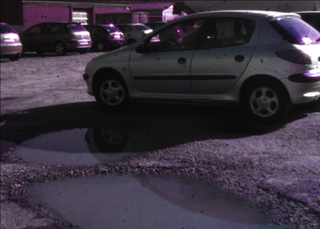
\includegraphics[width=\linewidth]{Figures/Aug/hsl.png}
	\end{subfigure}
	\begin{subfigure}[b]{0.32\linewidth}  
		\centering 
		\caption*{Rotated Image}
		
		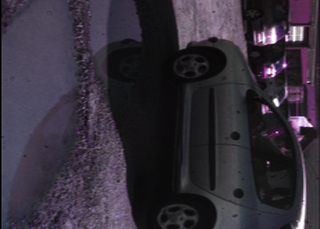
\includegraphics[width=\linewidth]{Figures/Aug/hsl_trans_rot.png}
	\end{subfigure}
	\begin{subfigure}[b]{0.32\linewidth}
		\centering
		\caption*{Regularized Image}
		
		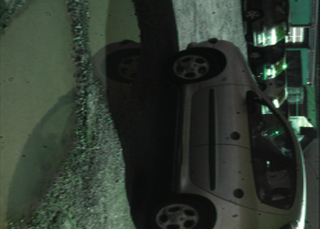
\includegraphics[width=\linewidth]{Figures/Aug/regularized_rot.png}
	\end{subfigure}

	\caption{Step-by-step rotation applied to polarimetric image.}\label{rotreal}
\end{figure}

Since the general idea is to reobtain the viability of the scene physics, this regularization step reorganizing the pixels of the DoFP grid is mandatory. However, as shown in the Figure \ref{rotreal}, this operation impacts the visual of the image. As shown in the Section \ref{rep_pol}, the images are modulated on the HSL model. As a reminder, we indexed the $\alpha$ polarization angle on the Hue channel, or more directly the color. Since the equation \ref{eq:Rot} applies a modification on this channel, then the global hue of the image changes. This is consistent with the fact that the change in pose implies a reorientation of all angles. To guarantee the periodicity of the angle but also to respect the HSL format, an additional modulo step is necessary:
\begin{equation}\label{eq:mod}
H_{final} = H_{transformed} \pmod{360}
\end{equation} 

As a partial conclusion, it is possible to deduce this operation is valid and respects the modality thanks to this visual indicator. In addition, the equation \ref{eq:mod} allows a correct bounding as well as taking advantage of the HSL mode. Thus, any rotation is applicable without altering the information.

In addition, the rotation represent a physically verifiable operation. It does not imply an impossible transformation to the sensor and therefore it is possible to verify the viability of the regularization by performing acquisitions.
As shown in the Figure \ref{proofexper}, this manipulation was performed to physically verify if the polarization information maintained by our equation.

\begin{figure}[h]
	\centering
	\begin{subfigure}[b]{0.3\linewidth}  
		\centering 
		\caption{Acquisition 0$^\circ$}
		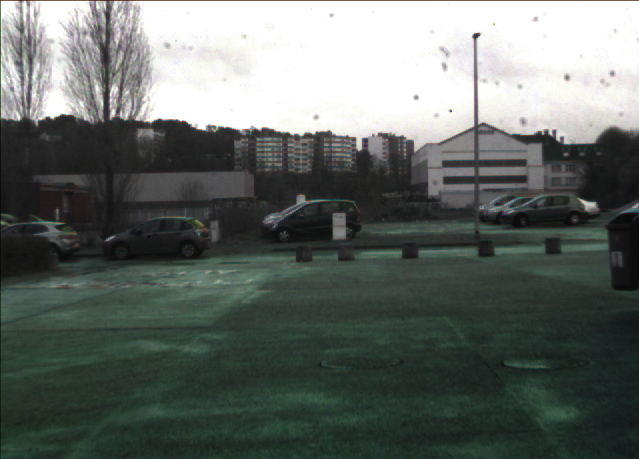
\includegraphics[width=\linewidth]{Figures/Aug/exprimentalTest/phys0.png}
	\end{subfigure}
	\begin{subfigure}[b]{0.3\linewidth}   
		\centering 
		\caption{Acquisition 90$^\circ$}
		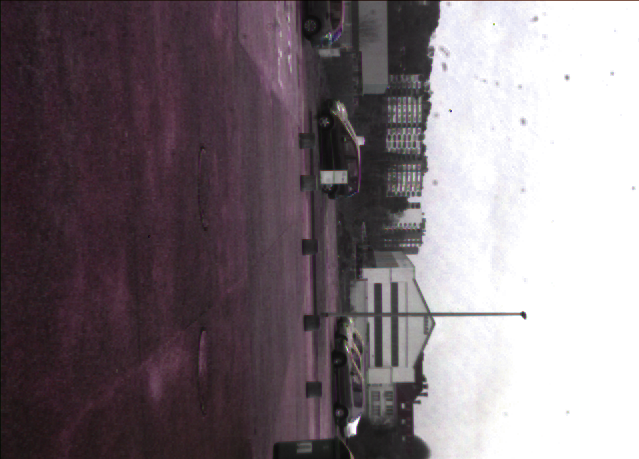
\includegraphics[width=\linewidth]{Figures/Aug/exprimentalTest/phys90.png}
	\end{subfigure}
	\begin{subfigure}[b]{0.3\linewidth}   
		\centering 
		\caption{Augmented 90$^\circ$}
		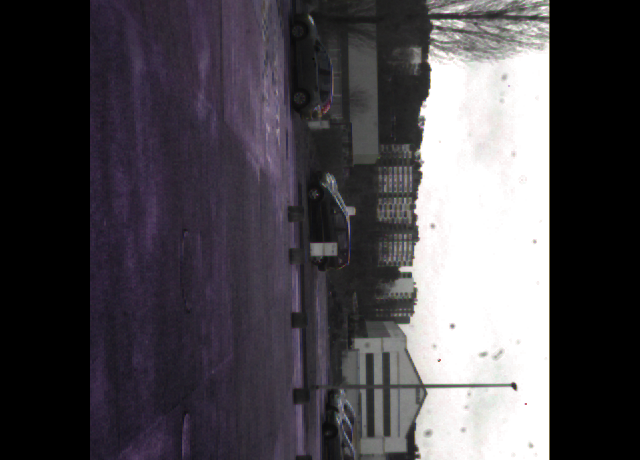
\includegraphics[width=\linewidth]{Figures/Aug/exprimentalTest/augmented.png}
	\end{subfigure}
	\caption[Experimental validation of rotation process.]{Experimental validation of rotation process.  Images (A) and (B) are acquisitions with physical rotations applied to the camera. Image (C) is the result of augmentation applied to image (A). Note the correct recovery of angle information.
	}\label{proofexper}
\end{figure}

The experimentation consists simply of two acquisitions. One image is captured with the camera oriented normally and a second one with a rotation of 90$^\circ$. We can then perceive the change in hue that this rotation implies. In addition, we can use the non-rotated image and transform it using our process. Thus, we obtain two images: one where the sensor has been physically rotated, and the other that has been artificially rotated.
Subsequently, it is possible to see the shades are approximately the same. A difference is present, but this is due to the parallax effect (imperfect rotation around the depth axis) and since the sensor used is not square. Nevertheless, this experiment shows the validity of the rotation process applied to polarimetry.

In conclusion, this experimental proof validates the rotation process and its associated regularization equation.



\subsection{Symmetry}\label{syn}

Symmetry is another frequently used transformation for augmentation. It allows "disorienting" the algorithms so that they do not get used to positional criteria, much like rotation.
The significant drawback of this transformation is that, unlike rotation, it is not physically verifiable. It goes without saying it is impossible to reverse the scene or to turn the sensor on itself.
This is why we have developed a method to express the impact of this operation and thus validate it.

\begin{figure}[h]
	\centering
	\begin{subfigure}[b]{0.29\linewidth}
		\centering
		\caption*{\footnotesize Base Image}
		
		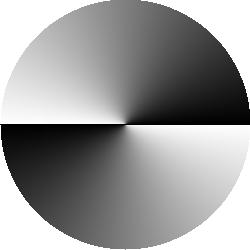
\includegraphics[width=\linewidth]{Figures/Aug/grad.jpg}
	\end{subfigure}
	\begin{subfigure}[b]{0.29\linewidth}  
		\centering 
		\caption*{\footnotesize Flipped Image}
		
		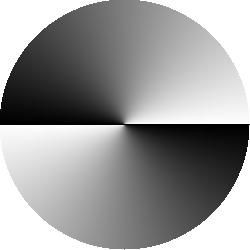
\includegraphics[width=\linewidth]{Figures/Aug/flipped.jpg}
	\end{subfigure}
	\begin{subfigure}[b]{0.29\linewidth}
		\centering
		\caption*{\footnotesize Regularized Image}
		
		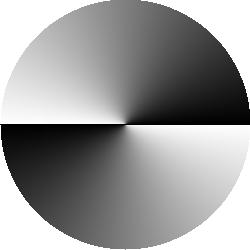
\includegraphics[width=\linewidth]{Figures/Aug/grad.jpg}
	\end{subfigure}
	\caption[Illustration of the flipping procedure.]{Illustration of the flipping procedure. From left to right, the base image, a flipped image and the regularized image}\label{flipreadtheo}
\end{figure}
The figure \ref{flipreadtheo} shows a circle separated into two halves.
This illustration is specific because each point of the circle in the image represents the corresponding angle with the center as reference.
If we consider only the top of the left circle, from left to right, we have a circular gradient ranging from 180 degrees to 0 degrees. Therefore, this image represents the full range of possible linear polarization angles in an image.
Knowing that the image hue channel is periodic at 360 degrees, the reversal consists of inverting the axis selected for the transformation.
Taking advantage of the periodicity of the angle and the selected format, then the transformation can be performed as follows:

\begin{equation}\label{eq:flip}
H_{\textrm{flipped}} = -H_{prev}.
\end{equation} 

Clearly, the physical operation of flipping is operated on the image in addition to regularization.
Thanks to the equation \ref{eq:mod} in addition to equation \ref{eq:flip}, we possess the possibility to use the representation mode to our advantage. This operation makes the format valid and thus, the accumulation of these two manipulations is necessary to verify the simulation proposed in figure \ref{flipreadtheo}.
Finally, the equation has this double role of regularization for symmetry and buffer to guarantee the validity of the color space.


\begin{figure}[h]
	\centering

	\begin{subfigure}[b]{0.32\linewidth}
		\centering
		\caption*{Base Image}
		
		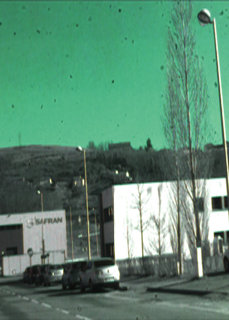
\includegraphics[width=\linewidth]{Figures/Aug/hsl_flip.png}
	\end{subfigure}
	\begin{subfigure}[b]{0.32\linewidth}  
		\centering 
		\caption*{Flipped Image}
		
		\scalebox{-1}[1]{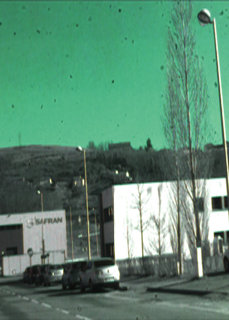
\includegraphics[width=\linewidth]{Figures/Aug/hsl_flip.png}}
	\end{subfigure}
	\begin{subfigure}[b]{0.32\linewidth}
		\centering
		\caption*{Regularized Image}
		
		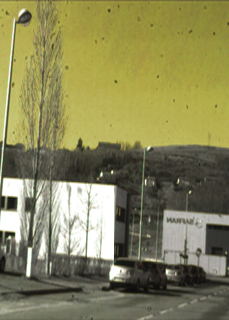
\includegraphics[width=\linewidth]{Figures/Aug/regularized_flipped.png}
	\end{subfigure}
	
	\caption[Flipping operation on real image and impact.]{Flipping operation on real image and impact. From left to right, initial image, the flipped image and the regularized image.}\label{flipread}
\end{figure}

It is then possible to perform these transformations on real images as shown in the figure \ref{flipread}.
Since it is impossible to physically observe this kind of transformation, the visual hue indexer will be the sole indicator of an integral transformation. Despite this, it is equally possible to check if the hue is well "inverted" by checking on the HSL representation space (shown in figure \ref{fig:hslrgb}) if the colors are properly symmetrical.

In conclusion, we note symmetry is another valid augmentation possibility to obtain realistic images of polarization thanks to our regularization process.


\subsection{Final procedure}\label{fin_proc}

In this part the final procedure of augmentation will be explained, but first of all a point must be addressed: what happens to the other channels.
Indeed, in the two previous parts on the different transformations, only the angle was modified. This can be explained by the invariance of the other two channels, the degree of polarization and the intensity, with respect to the pose.
The observation is simple, the reflection strength or the texture does not change according to the pose, such as, a reflective object remains reflective regardless of the camera orientation. Similarly, the texture is unaffected by a change in pose similarly to usual colorimetric image processing.
Thus, we conclude only the angle must undergo regularization operations while the other channels will only be affected by the rotation or flipping type transformation.



\begin{figure}[h]
	\centering
	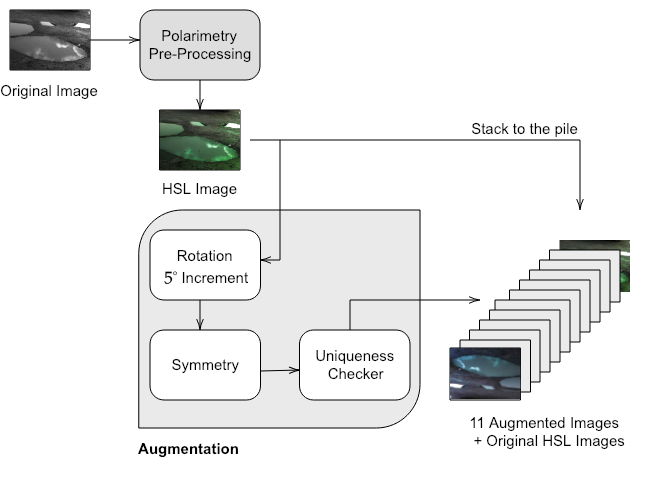
\includegraphics[width=.7\linewidth]{Figures/Aug/diagram-20190220.png}
	%\input{aug.tex}
	\caption[Illustration of the augmentation per image procedure.]{Illustration of the augmentation per image procedure. This process is repeated for each image in the original dataset to obtain a consistent large dataset. Then, the entire set of augmented images is shuffled.}\label{augment}
\end{figure}

This observation allowing to conclude on the augmentation pipeline, it is then possible to define the final process to augment the dataset.
Augmentation is typically composed of multiple operations performed simultaneously according to probabilistic or empirical rules. 
We therefore propose, with our transformations, to compose in the same way. Thus, we have the ability to cumulate rotation and flipping, at different increments or orientation.
As shown in the figure \ref{augment}, from a polarimetric image, we convert it to HSL as explained in Section \ref{rep_pol}. At that point in time, the image is randomly rotated by increments of 5$^\circ$ and flipped according to an empirically fixed probability. To complete the augmentation, our algorithm checks the uniqueness of the image to prevent redundancies and then converts these images in RGB format as expressed in Section \ref{rep_pol}.


At the end of this augmentation pipeline\footnote{Available at: \url{https://github.com/BlanchonMarc/P_Augmentor}}, starting from a unique image, it is possible to obtain $N$ physically correct polarimetric images. Following our numerous experiments, we concluded that 11 images generated with a unique image (i.e. 12 images in total as shown in the illustration) was sufficient to obtain enough images. 


Finally, implementing all these manipulations, we have proposed a new pipeline to perform augmentation operations on a physical-based modality, polarimetry.


\section{Network architectures}\label{net_4}

As a usefulness proof of polarization for the understanding of urban areas, we propose performing a benchmark comparing colorimetry and polarimetry, but also to approve the augmentation method presented in Section \ref{aug_4}.

Since one of the most widespread understanding applications is DL-based PwSS, we propose to perform this quantitative and qualitative study using proven architecture in literature.

\subsection{SegNet}\label{segnet_sec}

SegNet\cite{DBLP:journals/corr/BadrinarayananH15}, shown in Figure \ref{seg-arch}, is a simple architecture composed of an encoder and a decoder. Designed for scene segmentation and widely used with "city/road" datasets.  This network is not considered the state of the art but rather a pioneer in the field of PwSS.  It is notable for its small number of layers and simple composition (shown in the table \ref{tab:segnet}). 

\begin{figure}[h]
	\centering
	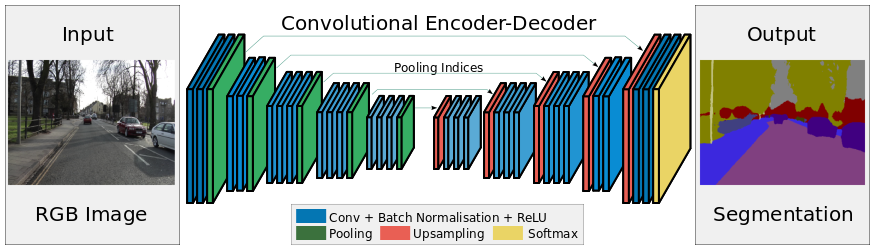
\includegraphics[width=\linewidth]{Figures/master-thesis/segnet.png}
	%\input{aug.tex}
	\caption{Illustation of SegNet architecture.}\label{seg-arch}
\end{figure}

The chief idea behind the emergence of this network as a point of comparison between RGB and Polarimetry is that it is not especially necessary to use overly complex networks. Indeed, the approach here is not principally to observe efficient results but to compare in the most unbiased way the ability to appreciate the scenes through different modalities. 
Thus, through this network, it is possible, with a simple encoder-decoder architecture, to focus on the modality and not on the performances that the network could infuse.


\begin{table}[h]
	\caption{Detailed SegNet architecture.}
	\centering
	\begin{adjustbox}{width=1\textwidth}
		\begin{tabular}{| c | c  c  c  c  c || c | c  c  c  c  c |}
			
			\toprule
			\multicolumn{6}{|c||}{\textbf{Encoder}}
			&
			\multicolumn{6}{|c|}{\textbf{Decoder}} \\\cline{1-6}\cline{7-12} 
			&\textbf{Type}&\textbf{Kernel}&\textbf{Padding}&\textbf{Stride}&\textbf{Output Depth}& &\textbf{Type}&\textbf{Kernel}&\textbf{Padding}&\textbf{Stride}&\textbf{Output Depth}\\\cline{1-6}\cline{7-12} 
			
			&conv1&3x3&1&1&Depth Image& &conv14&3x3&1&1&512\\
			\textbf{Block1}&conv2&3x3&1&1&64&\textbf{Block1d}&conv15&3x3&1&1&512\\
			& & & & & & &conv16&3x3&1&1&512\\\cline{1-6}\cline{7-12}
			
			&conv3&3x3&1&1&64& &conv17&3x3&1&1&512\\
			\textbf{Block2} &conv4&3x3&1&1&128&\textbf{Block2d}&conv18&3x3&1&1&512\\
			& & & & & & &conv19&3x3&1&1&256\\\cline{1-6}\cline{7-12}
			
			&conv5&3x3&1&1&128& &conv20&3x3&1&1&256\\
			\textbf{Block3}&conv6&3x3&1&1&256&\textbf{Block3d}&conv21&3x3&1&1&256\\
			&conv7&3x3&1&1&256& &conv22&3x3&1&1&126\\\cline{1-6}\cline{7-12}
			
			&conv8&3x3&1&1&256& &conv23&3x3&1&1&126\\
			\textbf{Block4}&conv9&3x3&1&1&512&\textbf{Block4d}&conv24&3x3&1&1&64\\
			&conv10&3x3&1&1&512& & & & & & \\\cline{1-6}\cline{7-12}
			
			&conv11&3x3&1&1&512& &conv25&3x3&1&1&64\\
			\textbf{Block5}&conv12&3x3&1&1&512&\textbf{Block5d}&conv26&3x3&1&1&Desired Depth\\
			&conv13&3x3&1&1&512& & & & & & \\
			\bottomrule
		\end{tabular}
	\end{adjustbox}
	\vspace{0.5ex}
	\label{tab:segnet}
\end{table}


\subsection{DeepLab V3+}\label{deeplab_sec}

DeepLab v3+\cite{chen2017rethinking}, shown in Figure \ref{deeplab-fig}, is much more advanced compared to SegNet. Indeed, its complex design composed of atrous convolution and ASPP (these two concepts are explained in the Chapter) is much more powerful than the previous architecture. 
\begin{figure}[h]
	\centering
	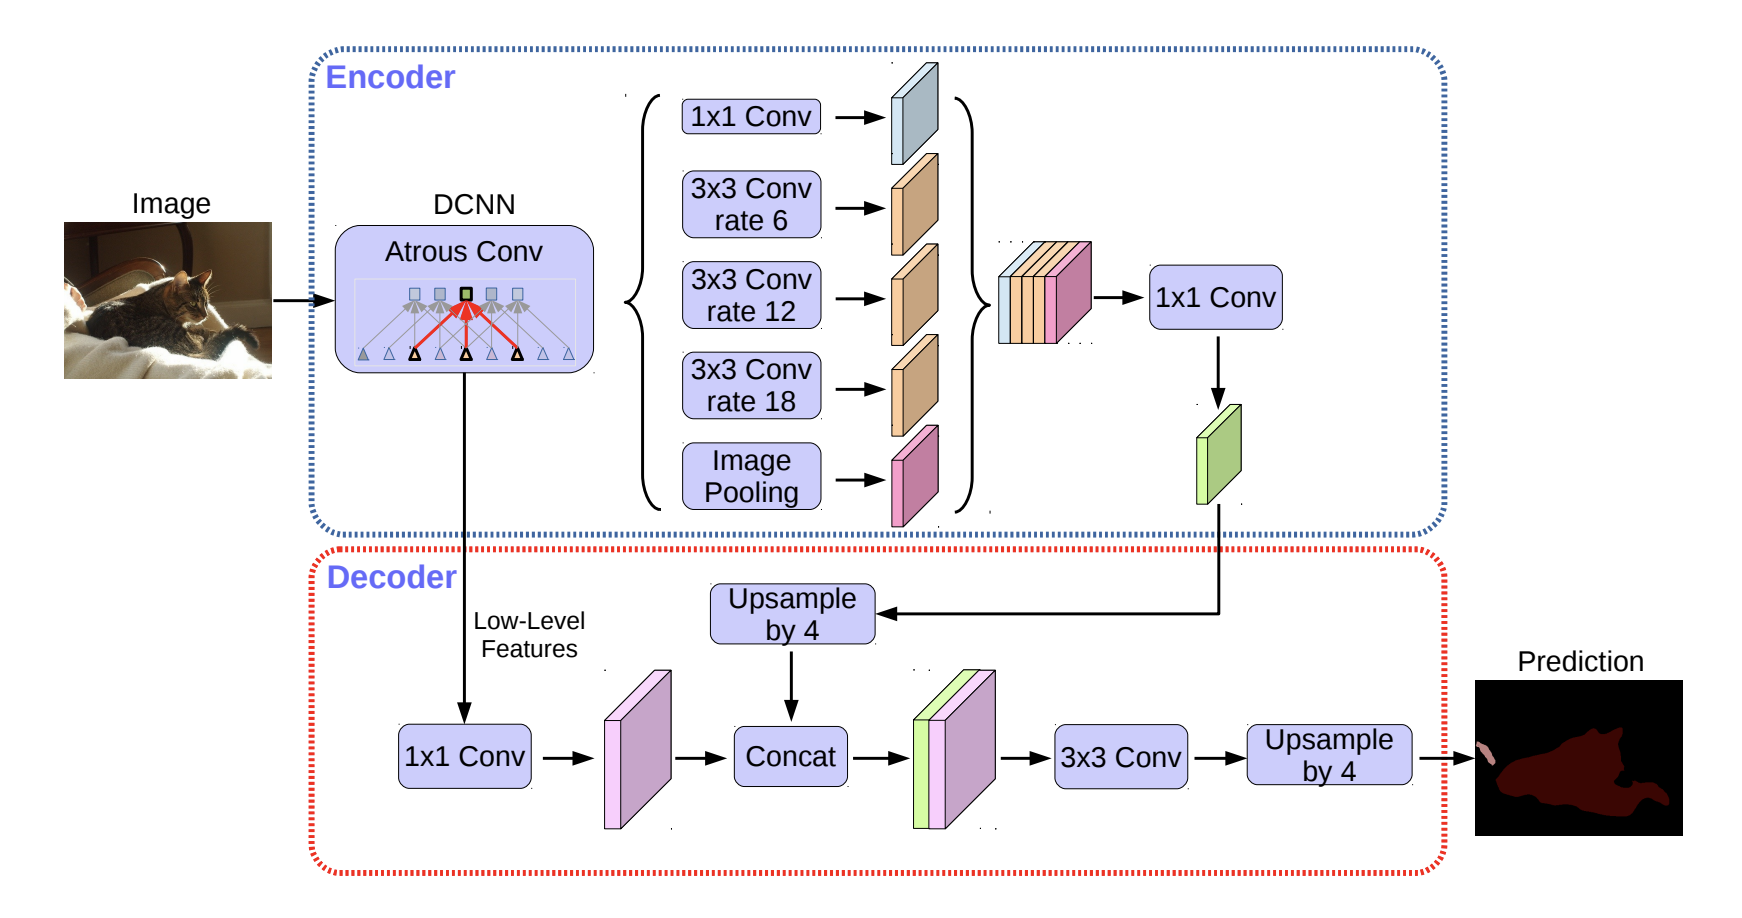
\includegraphics[width=\linewidth]{Figures/DL/deeplab-arch.png}
	%\input{aug.tex}
	\caption[Illustation of DeepLab V3+ architecture.]{Illustation of DeepLab V3+ architecture. Schematic borrowed from \cite{chen2017rethinking}.}\label{deeplab-fig}
\end{figure}


The use of such a network is motivated by the need to quantify the utility of the augmentation in favorable situations. Indeed, by implementing a complex architecture, it is possible to benefit the learning of complex features and in this case, the physical validity of polarimetry. 
In this manner, it will be possible to quantify the usefulness and/or the necessity of the augmentation.



\section{Experiments}\label{exp_4}

The experiments conducted allow two independent scopes.


On one hand, a series of experiments is focused on the differences of modalities. The prime goal of this set is to demonstrate the interest of polarization over colorimetry. The idea is to prove that with the same comparison method, a alternative form of information sustains a considerable interest for some fields. Therefore, without needing to unnecessarily increase the complexity of the processing cores, it is possible to reach satisfactory results.


In a second step, we propose to investigate the usefulness of an augmentation adapted to a physics-based modality. Here, in order for the algorithm to grasp maximum advantage of the available information (valid or invalid), we use a state-of-the-art DCNN. 

\subsection{Modality-based Comparison}

In this section, our proposal is to compare the modalities on the same basis, using aligned images, representing the same scenes.
We manipulate the non-augmented images from PolaBot (see Section \ref{data_pol}) and the network presented in Section \ref{segnet_sec}.

The images presented to the network show urban scenes that are conducive to reflection. As a reminder, we assume a large number of objects are reflective in urban areas such as: cars, windows or wet roads.
Thus, to highlight the respective capabilities of the networks trained jointly with colorimetry and polarimetry, the images were manually annotated with eight particular classes.
These eight classes designed for autonomous robotics are: Buildings (gray), Car (red), Road (orange), Sky (green), Water (blue), Window (light yellow), None (white) and Unlabeled (black). These classes are clearly differentiated by their segmented color and were determined for their interest in complex areas but also because they can lead to confusion with standard sensors. Also, the None class represents all the areas that have been judged uninterestingly for our comparison (e.g. trees, sidewalks,...) and the Unlabeled class comes from manual annotation errors.


Therefore, a simple metric, allowing an explicit comparison, was chosen. Indeed, the accuracy per class has been defined as:


\begin{equation}
\textrm{Accuracy}_C = \frac{\sum \; ^pP_C}{\sum \; ^gP_C},
\end{equation}

with C the class, $^pP_C$ the correctly predicted pixel of the class C and $^gP_C$ the ground truth pixel of class C.

For the training procedure, the construction of the dataset (explained in previous section) allows for pre-training and therefore the use of transfer learning\cite{torrey2010transfer,pan2009survey} to help convergence and benefit from efficient previous training. Therefore, both networks have been pre-trained using VGG16. 
This process, in addition to being advantageous, will allow us both to verify if the HSL to RGB approach is valid but also to see the adaptation capabilities of the network to a physics-based modality although pre-trained with colorimetry.

\subsubsection{Results}

Since the training procedure was identical in the hyperparameters as well as in the order of appearance of the images, it is possible to quantitatively compare the results between the two modalities.


As shown in Figure \ref{fig:resultspwss}, the qualitative results seem almost identical. However, when analyzing Table \ref{AccDiff}, a significant difference appears in favor of polarization. 

\begin{figure}[!htb]
\captionsetup{width=\linewidth}	
\begin{minipage}{0.48\textwidth}
		\captionsetup{width=.8\linewidth}
		\centering
		\begin{subfigure}[b]{0.3\linewidth}
			\reflectbox{\rotatebox[origin=c]{180}{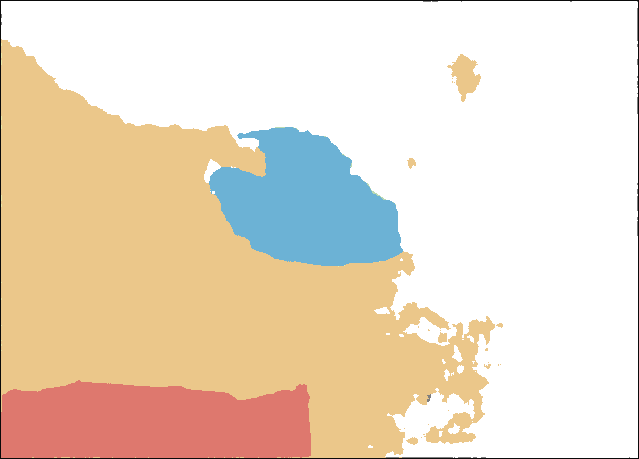
\includegraphics[width=\linewidth]{Figures/VISAPP/1pred.png}}}
		\end{subfigure}
		\begin{subfigure}[b]{0.3\linewidth}
			\reflectbox{\rotatebox[origin=c]{180}{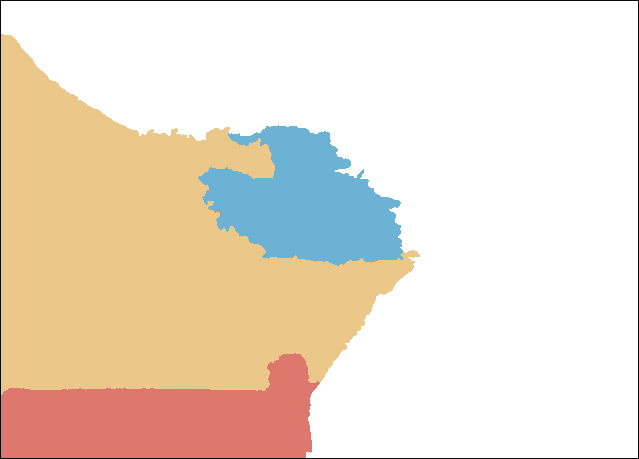
\includegraphics[width=\linewidth]{Figures/VISAPP/1gt.png}}}
		\end{subfigure}
		\begin{subfigure}[b]{0.3\linewidth}
			\reflectbox{\rotatebox[origin=c]{180}{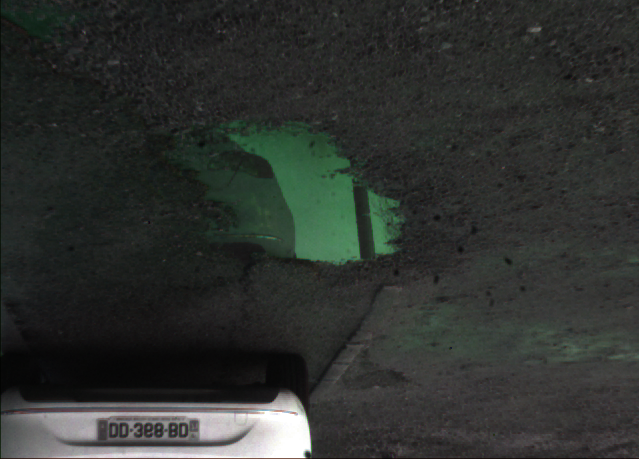
\includegraphics[width=\linewidth]{Figures/VISAPP/1int.png}}}
		\end{subfigure}\\
		\begin{subfigure}[b]{0.3\linewidth}
			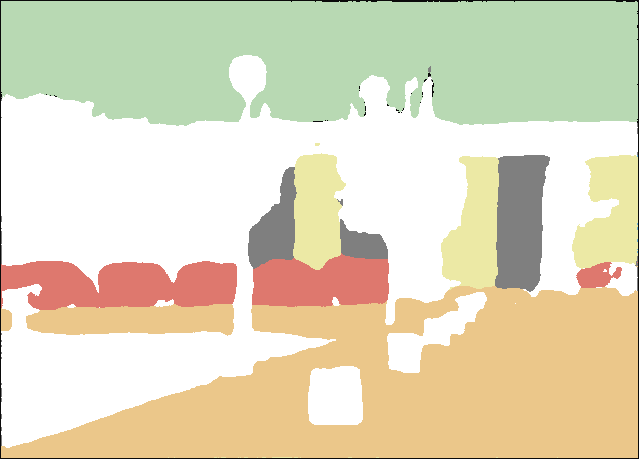
\includegraphics[width=\linewidth]{Figures/VISAPP/49pred.png}
		\end{subfigure}
		\begin{subfigure}[b]{0.3\linewidth}
			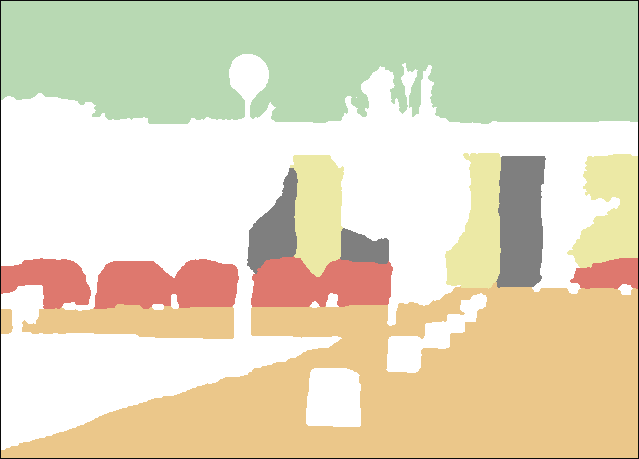
\includegraphics[width=\linewidth]{Figures/VISAPP/49gt.png}
		\end{subfigure}
		\begin{subfigure}[b]{0.3\linewidth}
			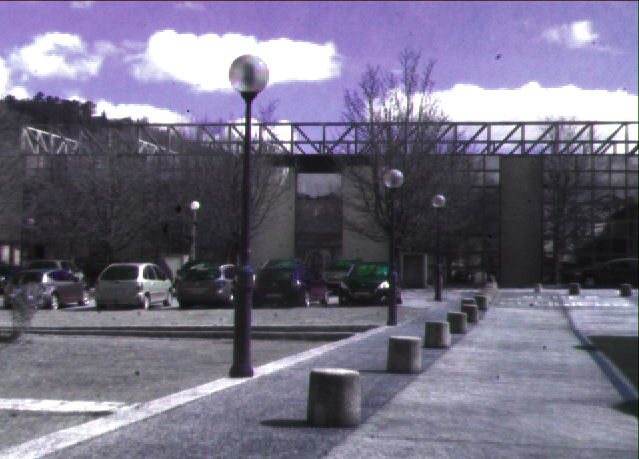
\includegraphics[width=\linewidth]{Figures/VISAPP/2int.png}
		\end{subfigure}\\
		\begin{subfigure}[b]{0.3\linewidth}
			\reflectbox{\rotatebox[origin=c]{180}{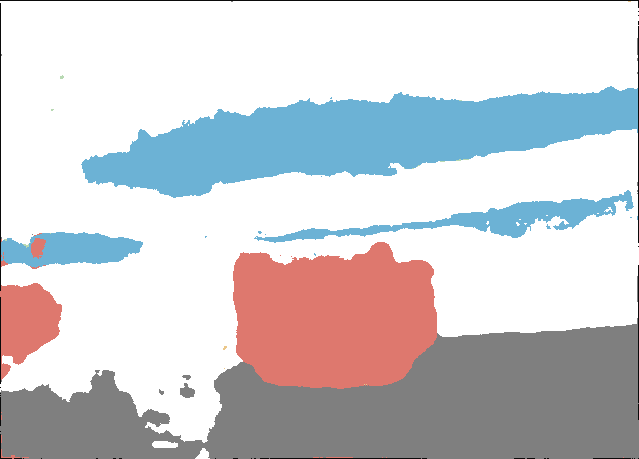
\includegraphics[width=\linewidth]{Figures/VISAPP/313pred.png}}}
		\end{subfigure}
		\begin{subfigure}[b]{0.3\linewidth}
			\reflectbox{\rotatebox[origin=c]{180}{
\includegraphics[width=\linewidth]{Figures/VISAPP/313gt.png}}}
		\end{subfigure}
		\begin{subfigure}[b]{0.3\linewidth}
			\reflectbox{\rotatebox[origin=c]{180}{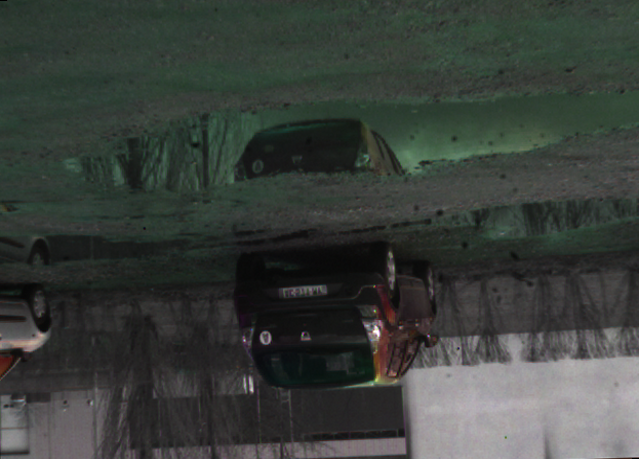
\includegraphics[width=\linewidth]{Figures/VISAPP/5int.png}}}
		\end{subfigure}		
		\subcaption{Polarimetry PwSS qualitative results.}
		\label{fig:polares}	
\end{minipage}
\hfill
\begin{minipage}{0.48\textwidth}
		\captionsetup{width=\linewidth}	
		\centering
		\begin{subfigure}[b]{0.3\linewidth}
			\reflectbox{\rotatebox[origin=c]{180}{
\includegraphics[width=\linewidth]{Figures/VISAPP/1predrgb.png}}}
		\end{subfigure}
		\begin{subfigure}[b]{0.3\linewidth}
			\reflectbox{\rotatebox[origin=c]{180}{
\includegraphics[width=\linewidth]{Figures/VISAPP/1gtrgb.png}}}
		\end{subfigure}
		\begin{subfigure}[b]{0.3\linewidth}
			\reflectbox{\rotatebox[origin=c]{180}{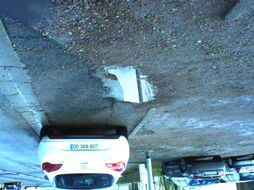
\includegraphics[width=\linewidth]{Figures/VISAPP/11int.png}}}
		\end{subfigure}\\
		\begin{subfigure}[b]{0.3\linewidth}
			\reflectbox{
\includegraphics[width=\linewidth]{Figures/VISAPP/55predrgb.png}}
		\end{subfigure}
		\begin{subfigure}[b]{0.3\linewidth}
			\reflectbox{
\includegraphics[width=\linewidth]{Figures/VISAPP/55gtrgb.png}}
		\end{subfigure}
		\begin{subfigure}[b]{0.3\linewidth}
			\reflectbox{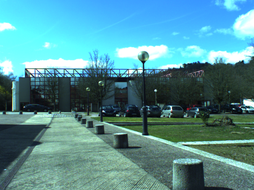
\includegraphics[width=\linewidth]{Figures/VISAPP/12int.png}}
		\end{subfigure}\\
		\begin{subfigure}[b]{0.3\linewidth}
			\reflectbox{\rotatebox[origin=c]{180}{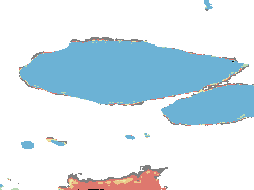
\includegraphics[width=\linewidth]{Figures/VISAPP/25predrgb.png}}}
		\end{subfigure}
		\begin{subfigure}[b]{0.3\linewidth}
			\reflectbox{\rotatebox[origin=c]{180}{
\includegraphics[width=\linewidth]{Figures/VISAPP/25gtrgb.png}}}
		\end{subfigure}
		\begin{subfigure}[b]{0.3\linewidth}
			\reflectbox{\rotatebox[origin=c]{180}{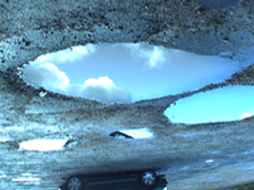
\includegraphics[width=\linewidth]{Figures/VISAPP/15int.png}}}
		\end{subfigure}
		\subcaption{Colorimetry PwSS qualitative results.}
		\label{fig:rgbres}	
\end{minipage}

\caption[Qualitative results comparing colorimetry and polarimetry with identical scenes.]{Qualitative results comparing colorimetry and polarimetry with identical scenes. For both the montages, respectively from left to right the images are: prediction, ground truth and input.}\label{fig:resultspwss}
\end{figure}



\begin{table}[h]
	\centering
	\caption{PwSS quantitative results comparing polarimetry and RGB.}
	\label{AccDiff}
	\resizebox{1\textwidth}{!}{
	\begin{tabular}{c|c|c|c|c|c|c|c||c|c|}
		\cline{2-9}
		& \textcolor{sky}{Sky} & \textcolor{water}{Water} & \textcolor{windows}{Windows} & \textcolor{road}{Road} & \textcolor{car}{Cars} & \textcolor{buildings}{Building} & \textcolor{none}{None} & Mean \\ \cline{2-8} \hline
		\multicolumn{1}{|c|}{Polarimetry} & 75.34 \%                    & 75.70 \%                      & 82.85 \%                       & 77.82 \%                     & 71.40 \%                    & 87.69 \%                         & 78.95 \% & 78.54 \%                    \\ \hline
		\multicolumn{1}{|c|}{RGB} & 89.57 \% & 78.61 \% & 44.50 \% & 78.45 \% & 48.48 \% & 67.84 \% & 83.4 \% & 69.83 \%                    \\ \hline \hline
		\multicolumn{1}{|c|}{Difference}  & -14.23\% & -3.51 \% & 38.35 \% & -0.63 \% & 22.92 \% & 19.85 \% & -4.45 \%  & 8.71 \%                  \\ \hline
	\end{tabular}}
	
\end{table}

Indeed, the accuracy per class shows with a network trained with polarimetric information, windows, cars and buildings are recognized in a better way. Moreover, the mean column shows a significant improvement compared to the identical algorithm using colorimetry.


\subsubsection{Discussion}

After numerous experiments and despite a fair comparison, the polarization-based approach seems to be more appropriate for the PwSS of complex urban scenes compared to colorimetry. Indeed, the use of polarization as a disciminant factor upstream of the network shows that for certain specificities, this information is more robust. 
It should be noted that the dataset was designed to highlight these DCNN behaviors which may partially explain the increased performance. Nevertheless, despite these advantages, polarization has proved its value. However, there is up until now an issue of data availability and consequently, the lack of consistent datasets.

This experiment also showed that DCNNs was able to adapt to supplementary information and that we could use transfer learning to rely only on fine-tuning. Moreover, the two methods compared having identical training, the learning on polarization emphasized a faster convergence. 

On the other hand, in the wrong direction, polarization was supposed to have a significant advantage over the Sky class since it is polarized. One possible explanation is the color makes it easy to discern the blue of the sky. Indeed, after experimentation, the dataset was found to be biased by this fact and in every image showing sky, it was blue. Thus, this is in our opinion the most plausible way to explain this performance which exceeds that of the polarization-based network.

To conclude this discussion, it is significant to note that polarization offers a substantial advantage for certain applications and especially for recognizing areas prone to reflection. Regrettably, the data is relatively rare and therefore not widely available. Nevertheless, through these experiments, it has been shown that a network is not only capable of learning from physics-based images but also that it is beneficial. Even with limited data, the comparisons emphasized the increased capabilities when the learning was conducted with this unconventional data.

\subsection{Augmentation-based Comparison}\label{abc}

Now that it has been established, that polarization-based algorithms tends to show increased performance in complex urban areas; this section will allow a study of the augmentation and its impact.
Indeed, the key idea is to show the interest of increasing the polarimetric image dataset by using the physics-friendly transforms established in section \ref{aug_4}.
Hence the use of an efficient network theoretically allowing a deeper use of the physical information of polarization.
The concept is to check if the augmentation is valid and its impact on the results. Thus, the experiment will be carried out using three different approach involving dataset: one will be not augmented, one augmented without using the regularization equations and a last implementing the augmentation presented in section \ref{aug_4}.
This approach allows a reliable comparison but also emphasizes the importance and even the necessity of an approach adapted to the modality.

\textbf{Encouraging segmented areas' expansion. } Usually, pixel segmentation techniques are discriminated using a simple loss chosen for its gradient behavior in logistic regression similar to the squared error loss for Linear regression. Indeed, the Cross entropy loss (CEL) allows to classify using probabilities and compare an outcome with a reality.
The multi-class CEL is defined as:

\begin{equation}
	CEL(x,c) = -log\Big( \frac{exp(x[c])}{\sum_j exp(x[j])} \Big) = -x[c] + log\Big( \sum_j exp(x[j]) \Big).
\end{equation}

While this feature is efficient, it tends to encourage pixel accuracy but neglects object logic. The fact is that the areas to be segmented are often plain surfaces and -outside of occlusion- do not have different classes. Thus, some applications, particularly medical imaging, opt for the use of the S\o rensen-Dice index (SDI). This one allows to encourage the propagation of a class and favors the fullness of the zones rather than considering only the pixel space. One could say SDI brings a more semantic dimension. This loss is defined as:

\begin{equation}
SDI =\frac{ \sum^{N}_{c} 1 - \frac{2 | X_c \cap Y_c|}{|X_c| + |Y_c|}}{N},\label{eq_dice}
\end{equation}

with  $X$  the label, $Y$ the prediction, $c$ the class and $N$ the number of classes. Since classes are unequally represented in the dataset, this metric allows an equal valuation of each of them unlike other losses.
Therefore, we will use the S\o rensen-Dice index for the training of the different networks since it allows us to obtain more satisfactory results semantically speaking.

\textbf{Metrics. }To effectively compare the diverse approaches and to evaluate the impact of the different augmentation methods, a comprehensive range of metrics were selected.
To effectively compare the different approaches and evaluate the impact of the different augmentation methods, a extensive range of metrics, defined in Appendix \ref{AppendixB}, has been selected. Thus, the \textit{IoU} was selected to quantify the overlap of the segmented areas with respect to the ground truth, the \textit{recall} and the \textit{precision} to measure respectively the consistency and the relevance of the segmentation. In addition, we chose to measure \textit{specificity} since it quantifies the ability to select and remove bad classes. This last metric allows us to verify if the segmentation is efficiently performed by zone and therefore SDI is meaningful for the application.



\subsubsection{Results}

As previously specified, three different DeepLab v3+ networks were trained with three different derivatives of the Polabot dataset.
These three networks will be named:

\begin{itemize}
	\item \emph{None:} for Polabot without any augmentation.
	\item \emph{Standard:} for Polabot augmented but without polarization angle regularization.
	\item \emph{Regularized:} for Polabot augmented and aggregated with the regularization presented in Section \ref{aug_4}.
\end{itemize}

The Standard or Regularized augmentation are both identical in the transformations oapplied n the images. This procedure, whether regularized or not, allows to obtain 2136 images from 178 (i.e. a 12/1 ratio).
In addition, an evaluation was performed based on whether or not the xception subnetworks were pre-trained using provided model\footnote{\url{https://data.lip6.fr/cadene/pretrainedmodels/}}.

As a recall, the scenes correspond to urban areas with seven different classes:

	\mbox{\textit{Road} (\textcolor{road}{dark yellow/orange})}, \textit{Buildings} (\textcolor{buildings}{grey}), \textit{Cars} (\textcolor{car}{red}), \textit{Water} (\textcolor{water}{blue}), \textit{Windows} (\textcolor{windows}{light yellow}), \textit{Sky} (\textcolor{sky}{green}) and \textit{None} (\textcolor{none}{light grey}).

\begin{figure}[h]
	\centering
	\begin{subfigure}[b]{0.3\linewidth}
		\centering
		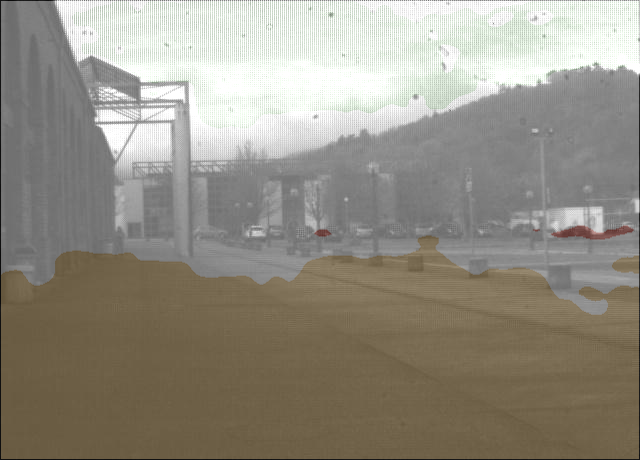
\includegraphics[width=\linewidth]{Figures/Aug/NA1/selected_images/overlayed/over0.png}
	\end{subfigure}
	\begin{subfigure}[b]{0.3\linewidth}  
		\centering 
		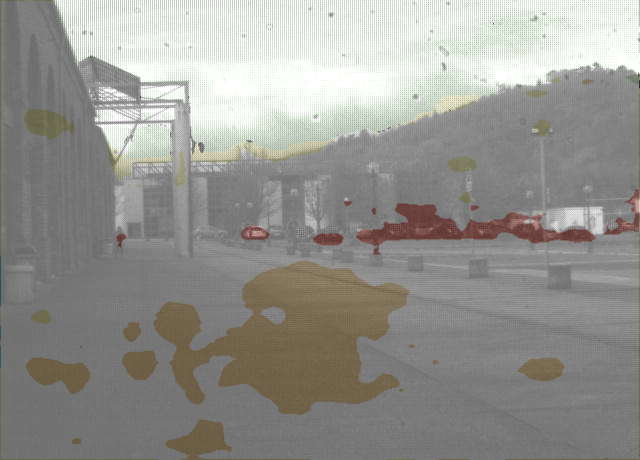
\includegraphics[width=\linewidth]{Figures/Aug/BA1/selected_images/overlayed/over0.png}
	\end{subfigure}
	\begin{subfigure}[b]{0.3\linewidth}  
		\centering 
		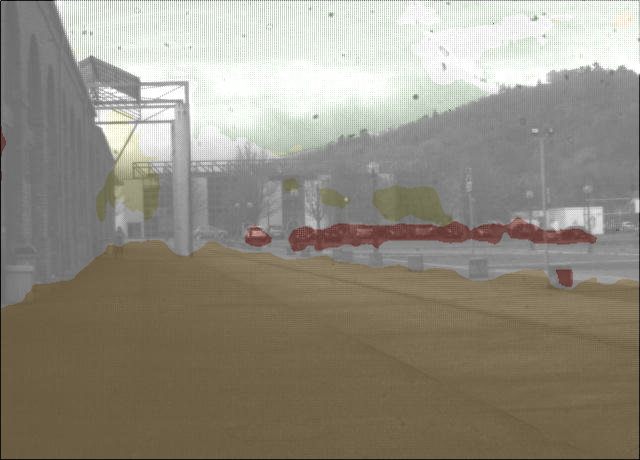
\includegraphics[width=\linewidth]{Figures/Aug/CA1/selected_images/overlayed/over0.png}
	\end{subfigure}
	\vskip\baselineskip
	\begin{subfigure}[b]{0.3\linewidth}  
		\centering 
		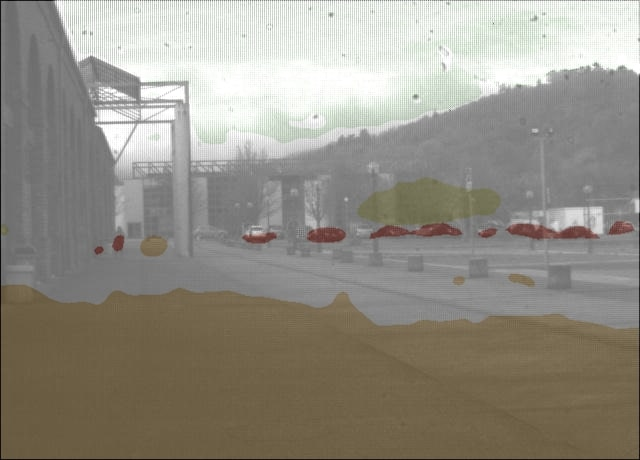
\includegraphics[width=\linewidth]{Figures/Aug/NA2/selected_images/overlayed/over0.jpg}
	\end{subfigure}
	\begin{subfigure}[b]{0.3\linewidth}  
		\centering 
		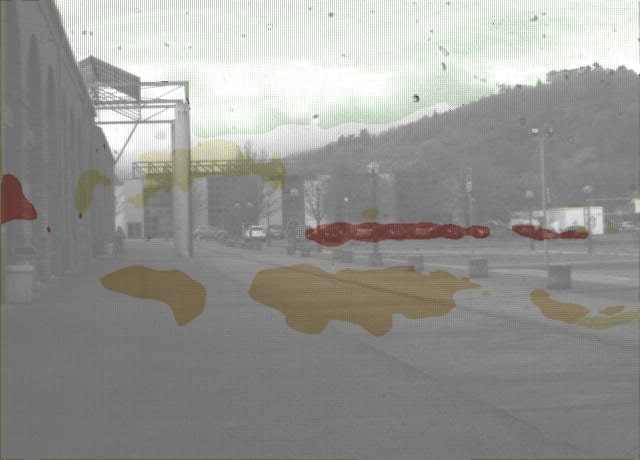
\includegraphics[width=\linewidth]{Figures/Aug/BA2/selected_images/overlayed/over0.jpg}
	\end{subfigure}
	\begin{subfigure}[b]{0.3\linewidth}  
		\centering 
		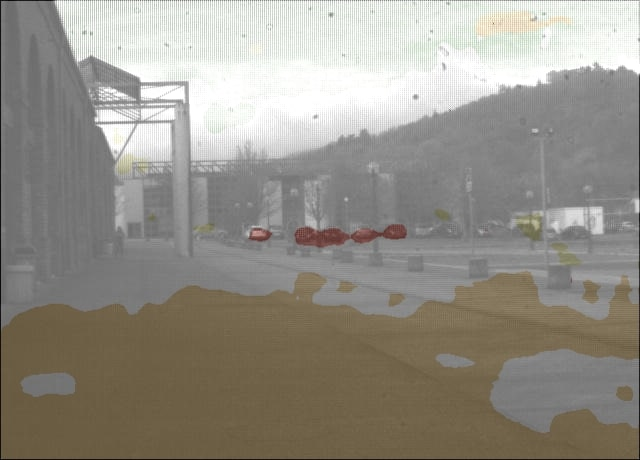
\includegraphics[width=\linewidth]{Figures/Aug/CA2/selected_images/overlayed/over0.jpg}
	\end{subfigure}
	\caption[Illustration of the diverse segmentation results obtained with different augmentation methods.]{Illustration of the diverse segmentation results obtained with different augmentation methods. The top line shows results for DeepLab v3+ network not pre-trained, and the bottom line the results with a pre-trained network. From left to right are presented predictions from networks trained with: un-augmented dataset, standarly augmented dataset and augmented dataset following our procedure. The four most representative segmented classes here are: \textit{Road} (\textcolor{road}{dark yellow/orange}), \textit{Cars} (\textcolor{car}{red}), \textit{Sky} (\textcolor{sky}{light green}) and \textit{None} (\textcolor{none}{light grey}). %In those images, some areas are badly segmented as windows (light yellow).
	}
	\label{comp1}
	\vspace{-0.25cm}
\end{figure}
As shown in Figure\ref{comp1}, for a same scene, 6 estimates are then proposed by the benchmark.



\begin{figure}[h]
	\centering
	
	\begin{subfigure}[b]{0.18\linewidth}   
		\centering 
		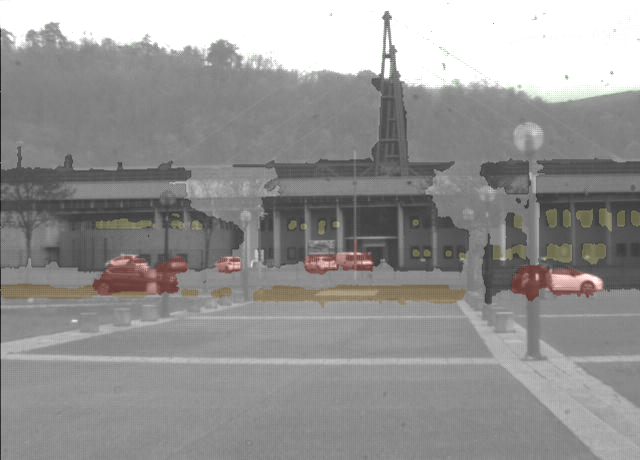
\includegraphics[width=\linewidth]{Figures/Aug/labels/overlayed/over1205.png}
	\end{subfigure}
	\begin{subfigure}[b]{0.18\linewidth}
		\centering
		\includegraphics[width=\linewidth]{Figures/Aug/labels/overlayed/over4427.png}
	\end{subfigure}
	\begin{subfigure}[b]{0.18\linewidth}  
		\centering 
		\includegraphics[width=\linewidth]{Figures/Aug/labels/overlayed/over4981.png}
	\end{subfigure}
	\begin{subfigure}[b]{0.18\linewidth}   
		\centering 
		\includegraphics[width=\linewidth]{Figures/Aug/labels/overlayed/over5142.png}
	\end{subfigure}
	\begin{subfigure}[b]{0.18\linewidth}   
		\centering 
		\includegraphics[width=\linewidth]{Figures/Aug/labels/overlayed/over5426.png}
	\end{subfigure}
	
	
	\vspace{0.1cm}
	
	
	\begin{subfigure}[b]{0.18\linewidth}   
		\centering 
		\includegraphics[width=\linewidth]{Figures/Aug/NA2/selected_images/overlayed/over1205.jpg}
	\end{subfigure}
	\begin{subfigure}[b]{0.18\linewidth}
		\centering
		\includegraphics[width=\linewidth]{Figures/Aug/NA2/selected_images/overlayed/over4427.jpg}
	\end{subfigure}
	\begin{subfigure}[b]{0.18\linewidth}  
		\centering 
		\includegraphics[width=\linewidth]{Figures/Aug/NA2/selected_images/overlayed/over4981.jpg}
	\end{subfigure}
	\begin{subfigure}[b]{0.18\linewidth}   
		\centering 
		\includegraphics[width=\linewidth]{Figures/Aug/NA2/selected_images/overlayed/over5142.jpg}
	\end{subfigure}
	\begin{subfigure}[b]{0.18\linewidth}   
		\centering 
		\includegraphics[width=\linewidth]{Figures/Aug/NA2/selected_images/overlayed/over5426.jpg}
	\end{subfigure}
	
	\vspace{0.1cm}  
	
	\begin{subfigure}[b]{0.18\linewidth}   
		\centering 
		\includegraphics[width=\linewidth]{Figures/Aug/BA2/selected_images/overlayed/over1205.jpg}
	\end{subfigure}
	\begin{subfigure}[b]{0.18\linewidth}
		\centering
		\includegraphics[width=\linewidth]{Figures/Aug/BA2/selected_images/overlayed/over4427.jpg}
	\end{subfigure}
	\begin{subfigure}[b]{0.18\linewidth}  
		\centering 
		\includegraphics[width=\linewidth]{Figures/Aug/BA2/selected_images/overlayed/over4981.jpg}
	\end{subfigure}
	\begin{subfigure}[b]{0.18\linewidth}   
		\centering 
		\includegraphics[width=\linewidth]{Figures/Aug/BA2/selected_images/overlayed/over5142.jpg}
	\end{subfigure}
	\begin{subfigure}[b]{0.18\linewidth}   
		\centering 
		\includegraphics[width=\linewidth]{Figures/Aug/BA2/selected_images/overlayed/over5426.jpg}
	\end{subfigure}
	
	\vspace{0.1cm} 
	
	
	\begin{subfigure}[b]{0.18\linewidth}   
		\centering 
		\includegraphics[width=\linewidth]{Figures/Aug/CA2/selected_images/overlayed/over1205.jpg}
	\end{subfigure}
	\begin{subfigure}[b]{0.18\linewidth}
		\centering
		\includegraphics[width=\linewidth]{Figures/Aug/CA2/selected_images/overlayed/over4427.jpg}
	\end{subfigure}
	\begin{subfigure}[b]{0.18\linewidth}  
		\centering 
		\includegraphics[width=\linewidth]{Figures/Aug/CA2/selected_images/overlayed/over4981.jpg}
	\end{subfigure}
	\begin{subfigure}[b]{0.18\linewidth}   
		\centering 
		\includegraphics[width=\linewidth]{Figures/Aug/CA2/selected_images/overlayed/over5142.jpg}
	\end{subfigure}
	\begin{subfigure}[b]{0.18\linewidth}   
		\centering 
		\includegraphics[width=\linewidth]{Figures/Aug/CA2/selected_images/overlayed/over5426.jpg}
	\end{subfigure}
	
	\caption[Examples of segmentation results according to the augmentation methods.]{Examples of segmentation results according to the augmentation methods. From top to bottom are present the ground-truth, then consecutively the results from model with pre-training with: no augmentation, standard augmentation and regularized augmentation.}
	\label{figres_aug}
\end{figure}

It is then possible to extract a range of images from the test dataset which is a video sequence comprised of 8,049 images acquired at a frequency of 10Hz sharing many characteristics with the training dataset.
Figure \ref{figres_aug}, shows a comprehensive panel of images representative of the results obtained from the various trainings.




\renewcommand{\arraystretch}{1.5}
\begin{table}[h]
	\centering
	
	\caption[Quantitative evaluation of augmentation procedures.]{Quantitative evaluation of augmentation procedures.Impact of the augmentation procedure on DeepLabV3+ network. Specific classes have been highlighted in relation to the robotic application to witness the obstacle-wise performance. Due to the limited training, \textit{Buildings} are almost undetected. For this reason, the averages denoted $\backslash B$ exclude the \textit{Buildings} class from the calculation. }\label{metriques}
	\large \center
	\resizebox{\textwidth}{!}{%
		\begin{tabular}{c|c|ccccc|ccccc|c|c}
			\multirow{2}{*}{\textbf{Augmentation}} & \multirow{2}{*}{\textbf{PreTraining}} & \multicolumn{5}{c|}{\textbf{IoU (\%)}}                                         & \multicolumn{5}{c|}{\textbf{Recall (\%)}}                                      & \multirow{2}{*}{\textbf{Precision (\%)}} & \multirow{2}{*}{\textbf{Specificity (\%)}} \\ \cline{3-12}
			&                                       & \textcolor{water}{@water}        & \textcolor{windows}{@windows}      & \textcolor{car}{@cars}         & Mean          & Mean $\backslash B$ & \textcolor{water}{@water}        & \textcolor{windows}{@windows}      & \textcolor{car}{@cars}         & Mean          & Mean $\backslash B$ &                                          &                                                            \\ \hline
			\multirow{2}{*}{None}                  & No                                    & 40.0          & 20.6          & 20.8          & 30.5          & 32.2           & 35.2          & 15.8          & 22.5          & \textbf{50.9} & 50.0           & 50.0                                     & 89.6                                                                           \\
			& Yes                                   & 54.0          & 10.3          & 43.46         & 33.5          & 34.8           & \textbf{42.4 }         & 15.3          & 57.4          & 43.3          & 50.3           & 50.1                                     & 91.0                                                                        \\ \hline
			\multirow{2}{*}{Standard}              & No                                    & 0.1           & 3.4           & 12.4          & 14.8          & 13.1           & 35.0          & 25.8          & 15.0          & 31.8          & 28.0           & 41.7                                     & 88.7                                                                        \\
			& Yes                                   & 10.2          & 3.0           & 19.7          & 21.8          & 20.0           & 35.2          & 22.9          & 23.4          & 37.0          & 33.4           & 41.2                                     & 91.2                                                                        \\ \hline
			\multirow{2}{*}{Regularized}           & No                                    & 63.9          & 13.3          & 46.7          & \textbf{43.4} & \textbf{50.3}  & 39.2 & 21.9          & \textbf{60.8} & 43.4          & \textbf{50.5}  & 48.5                                     & \textbf{91.3}                                                                \\
			& Yes                                   & \textbf{70.0} & \textbf{26.6} & \textbf{47.1} & 37.8          & 38.5           & 35.0          & \textbf{26.0} & 48.0          & 42.0          & 38.5           & \textbf{53.7}                            & 90.7                                                              
		\end{tabular}%
	}
	
\end{table}

Finally, each metric described above has been computed in order to compare quantitatively the different processes. Thus, Table \ref{metriques} shows the average performance of each pipeline. 

\subsubsection{Discussion}

The results, both quantitative and qualitative, show increased performance when using our method's proposed pipeline. It is quite clear that augmenting the data without taking into account the physical dimension of the images disrupts the capabilities of the network. In this sense, it is notable that according to our results, it is better not to increase the data and to keep an small amount of image rather than to augment naively. 
However, the augmented and regularized data allowed us to observe the best overall results.

In spite of these performances, the pre-training seems to have a significant impact. Indeed, when it is performed, then the results are significantly better and has a positive influence on the segmentation of the interest classes.

Finally, it is noticeable the adaptively augmented polarization allows a better recognition of the areas for which it has an advantage (i.e. the reflective areas). This is highlighted by the statistics calculated by interest class. This observation allows a second important conclusion. Networks, when using valid information, are able to take advantage of the physics and therefore can learn to interpret this new information.

The final important point to address is the augmentation procedure itself. When using conventional interpolable modalities, a broad extent of freedom is allowed. However, when using physics-based non-interpolable images, one must consider the factors defining the modality to size a customized augmentation. Thus, in addition to allowing for enhanced results, the augmentation, if it is made at all, must be tailored specifically for the type of imaging used.


\section{Summary}\label{sum_4}

In this chapter, our work involving polarization and pixel-wise semantic segmentation has been defined.
The polarimetric modality involving many dependencies has also oriented our work on more meta domains such as: dataset construction, representation choice and establishment of an adapted augmentation procedure.

The two different axes proposed have demonstrated the usefulness of this unconventional modality for the understanding of complex urban scenes. To be specific, a significant advantage was highlighted when colorimetry was put in competition with polarization. Therefore, our initial hypotheses on the ability to discern specular areas were verified by experimentation on our dataset designed for the occasion.
In addition, the augmentation procedure was validated following a meticulous evaluation which allowed the leverage of many constraints on the image volume requirements.

Furthermore, the effectiveness of deep learning-based polarization in urban scene understanding, which is a totally novel approach in the field, is demonstrated.

Ultimately, to appreciate the scenes from a geometric point of view, a polarization-based depth estimation pipeline will be elaborated in Chapter \ref{Chapter5}.


